\chapter{Full List of Features Invested}
\label{appendix:features}

For individual feature such as tm-pbs, $\checkmark$ indicates that the feature was used in the final model and $\times$ indicates that the feature was not used in the final model. At the same time, for a group of features, if at least one feature was used in the final model, a $\circ$ is placed in the last column. 

% table of features and their explanations
\begin{table}[ht]
    \centering
    \begin{tabular}{|p{0.3\textwidth}|p{0.5\textwidth}|p{0.1\textwidth}|}
        \hline
        \textbf{Feature} & \textbf{Explanation} & \textbf{Top 24} \\ 
        \hline
        tm-pbs& Melting temperature fo pbs RNA sequences & $\checkmark$ \\
        \hline
        tm-rt& Melting temperature of RT primer RNA sequences & $\times$ \\
        \hline
        tm-spacer& Melting temperature of spacer RNA sequences & $\checkmark$ \\
        \hline
        max-cas & Maximum number of consecutive A bases in the cDNA of extension as well as protospacer sequence & $\times$ \\
        \hline
        max-cts & Maximum number of consecutive T bases in the cDNA of extension as well as protospacer sequence & $\checkmark$ \\
        \hline
        max-cgs & Maximum number of consecutive G bases in the cDNA of extension as well as protospacer sequence & $\times$ \\
        \hline
        max-ccs & Maximum number of consecutive C bases in the cDNA of extension as well as protospacer sequence & $\times$ \\
        \hline
    \end{tabular}
\end{table}

% table of features and their explanations
\begin{table}[ht]
    \centering
    \begin{tabular}{|p{0.3\textwidth}|p{0.5\textwidth}|p{0.1\textwidth}|}
        \hline
        \textbf{Feature} & \textbf{Explanation} & \textbf{Top 24} \\ 
        \hline
        mfe-pbs & Minimum free energy of pbs RNA sequences & $\checkmark$ \\
        \hline
        mfe-rt & Minimum free energy of RT primer RNA sequences & $\times$ \\
        \hline
        mfe-spacer & Minimum free energy of spacer RNA sequences & $\checkmark$ \\
        \hline
    \end{tabular}
\end{table}

\chapter{Fine Tuning the Transformer Model}
\label{appendix:transformer-hyperparameter-tuning}

Full result of the hyperparameter tuning for the transformer model.

\begin{longtable}{|>{\raggedright\arraybackslash}p{2cm}|>{\raggedright\arraybackslash}p{2cm}|>{\raggedright\arraybackslash}p{2cm}|>{\raggedright\arraybackslash}p{3.5cm}|>{\raggedright\arraybackslash}p{2cm}|>{\raggedright\arraybackslash}p{2cm}|}
    \hline
    \textbf{MLP Embed Dim} & \textbf{Num Encoder Units} & \textbf{Dropout} & \textbf{Performance} & \textbf{Mean} & \textbf{Max} \\
    \hline
    \endfirsthead
    
    \hline
    \textbf{MLP Embed Dim} & \textbf{Num Encoder Units} & \textbf{P Dropout} & \textbf{Performance} & \textbf{Mean Performance} & \textbf{Max Performance} \\
    \hline
    \endhead
    
    \hline
    \endfoot
    
    100 & 1 & 0.1 & [0.8039, 0.8214, 0.8204, 0.7896, 0.7923] & 0.8055 & 0.8214 \\
    \hline
    100 & 1 & 0.3 & [0.8062, 0.8024, 0.8111, 0.8009, 0.8258] & 0.8093 & 0.8258 \\
    \hline
    100 & 1 & 0.5 & [0.7753, 0.7982, 0.7899, 0.8025, 0.7869] & 0.7906 & 0.8025 \\
    \hline
    100 & 2 & 0.1 & [0.8035, 0.8024, 0.7926, 0.8187, 0.7899] & 0.8014 & 0.8187 \\
    \hline
    100 & 2 & 0.3 & [0.8137, 0.8168, 0.8014, 0.7962, 0.7909] & 0.8038 & 0.8168 \\
    \hline
    100 & 2 & 0.5 & [0.7986, 0.8008, 0.7874, 0.7776, 0.7771] & 0.7883 & 0.8008 \\
    \hline
    100 & 3 & 0.1 & [0.7995, 0.8001, 0.8015, 0.8003, 0.8128] & 0.8028 & 0.8128 \\
    \hline
    100 & 3 & 0.3 & [0.7879, 0.8043, 0.7797, 0.7929, 0.7939] & 0.7917 & 0.8043 \\
    \hline
    100 & 3 & 0.5 & [0.7735, 0.7864, 0.7758, 0.7888, 0.7847] & 0.7818 & 0.7888 \\
    \hline
    150 & 1 & 0.1 & [0.8047, 0.8202, 0.8059, 0.8001, 0.7957] & 0.8053 & 0.8202 \\
    \hline
    150 & 1 & 0.3 & [0.8195, 0.8171, 0.8085, 0.7845, 0.7858] & 0.8031 & 0.8195 \\
    \hline
    150 & 1 & 0.5 & [0.7554, 0.7521, 0.7853, 0.7884, 0.7979] & 0.7758 & 0.7979 \\
    \hline
    150 & 2 & 0.1 & [0.7995, 0.8025, 0.7994, 0.7979, 0.7990] & 0.7996 & 0.8025 \\
    \hline
    150 & 2 & 0.3 & [0.7998, 0.7934, 0.7941, 0.8122, 0.8094] & 0.8018 & 0.8122 \\
    \hline
    150 & 2 & 0.5 & [0.7938, 0.7935, 0.7799, 0.7985, 0.7643] & 0.7860 & 0.7985 \\
    \hline
    150 & 3 & 0.1 & [0.8033, 0.7837, 0.8062, 0.8033, 0.8046] & 0.8002 & 0.8062 \\
    \hline
    150 & 3 & 0.3 & [0.7946, 0.7983, 0.7940, 0.8186, 0.7984] & 0.8008 & 0.8186 \\
    \hline
    150 & 3 & 0.5 & [0.7756, 0.7873, 0.7961, 0.7878, 0.7923] & 0.7878 & 0.7961 \\
    \hline
    200 & 1 & 0.1 & [0.8007, 0.8062, 0.8216, 0.8095, 0.8182] & 0.8112 & 0.8216 \\
    \hline
    200 & 1 & 0.3 & [0.7820, 0.8164, 0.7751, 0.8053, 0.8172] & 0.7992 & 0.8172 \\
    \hline
    200 & 1 & 0.5 & [0.7951, 0.7843, 0.7835, 0.7956, 0.8046] & 0.7926 & 0.8046 \\
    \hline
    200 & 2 & 0.1 & [0.8058, 0.7912, 0.7984, 0.8011, 0.7862] & 0.7965 & 0.8058 \\
    \hline
    200 & 2 & 0.3 & [0.7999, 0.7955, 0.7863, 0.8036, 0.7992] & 0.7969 & 0.8036 \\
    \hline
    200 & 2 & 0.5 & [0.7867, 0.7715, 0.7559, 0.7856, 0.7680] & 0.7735 & 0.7867 \\
    \hline
    200 & 3 & 0.1 & [0.8040, 0.8018, 0.8117, 0.8252, 0.8054] & 0.8096 & 0.8252 \\
    \hline
    200 & 3 & 0.3 & [0.8034, 0.7934, 0.7644, 0.8073, 0.7846] & 0.7906 & 0.8073 \\
    \hline
    200 & 3 & 0.5 & [0.7701, 0.7940, 0.7706, 0.7858, 0.7865] & 0.7814 & 0.7940 \\
    \hline
    \caption{Transformer model's performance using different hyperparameters controlling the parameter size. The hyperparameters are the MLP Embedding Dimension (number of hidden units in the positional feedforward network), Number of Encoder Units (number of transformer layers to stack), and the Dropout Rate. The raw performance as well as the mean and maximum performance are shown.} 
    \end{longtable}
    


\chapter{Additional Figures}
\label{appendix:additional-figures}

\section{Additional Figures for Error Analysis}
\label{appendix:error-analysis-figures}



\begin{figure}[ht]
    \centering
    \subfigure[][Error Distribution]{
        \centering
        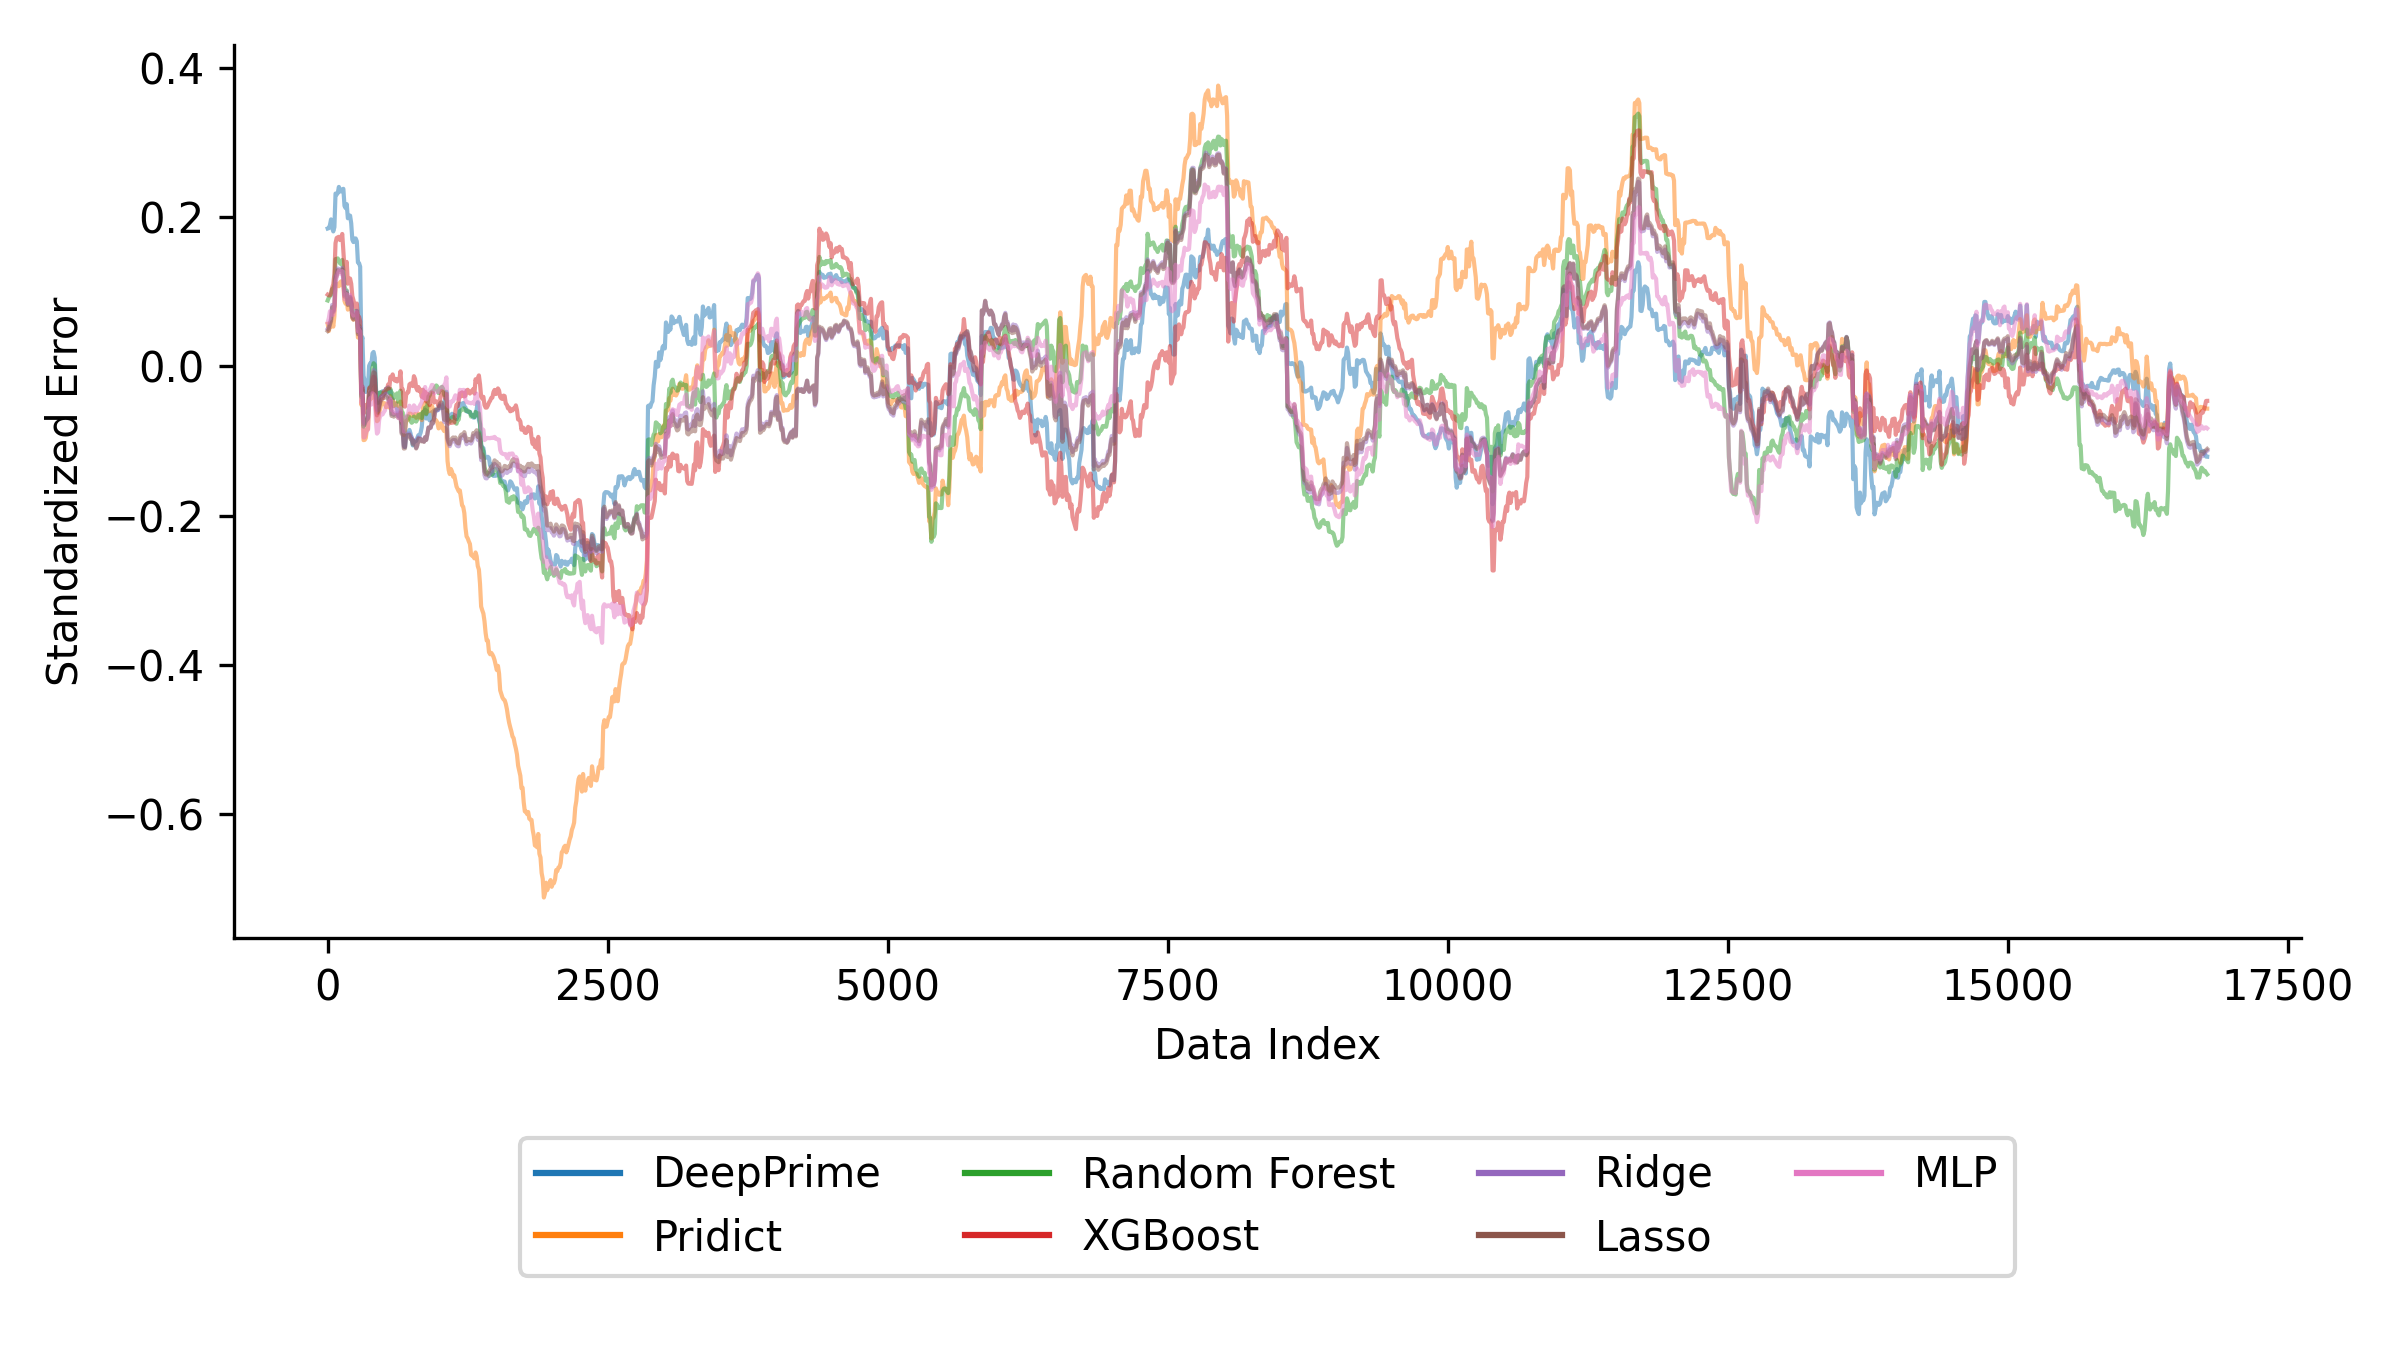
\includegraphics[width=\textwidth]{error_comparison_pd-adv-pe2.png}
        % \caption{Error Distribution of the Individual Models}
        \label{fig:error-distribution-adv-pe2}
    }
    \subfigure[][Pearson Correlation]{
        \centering
        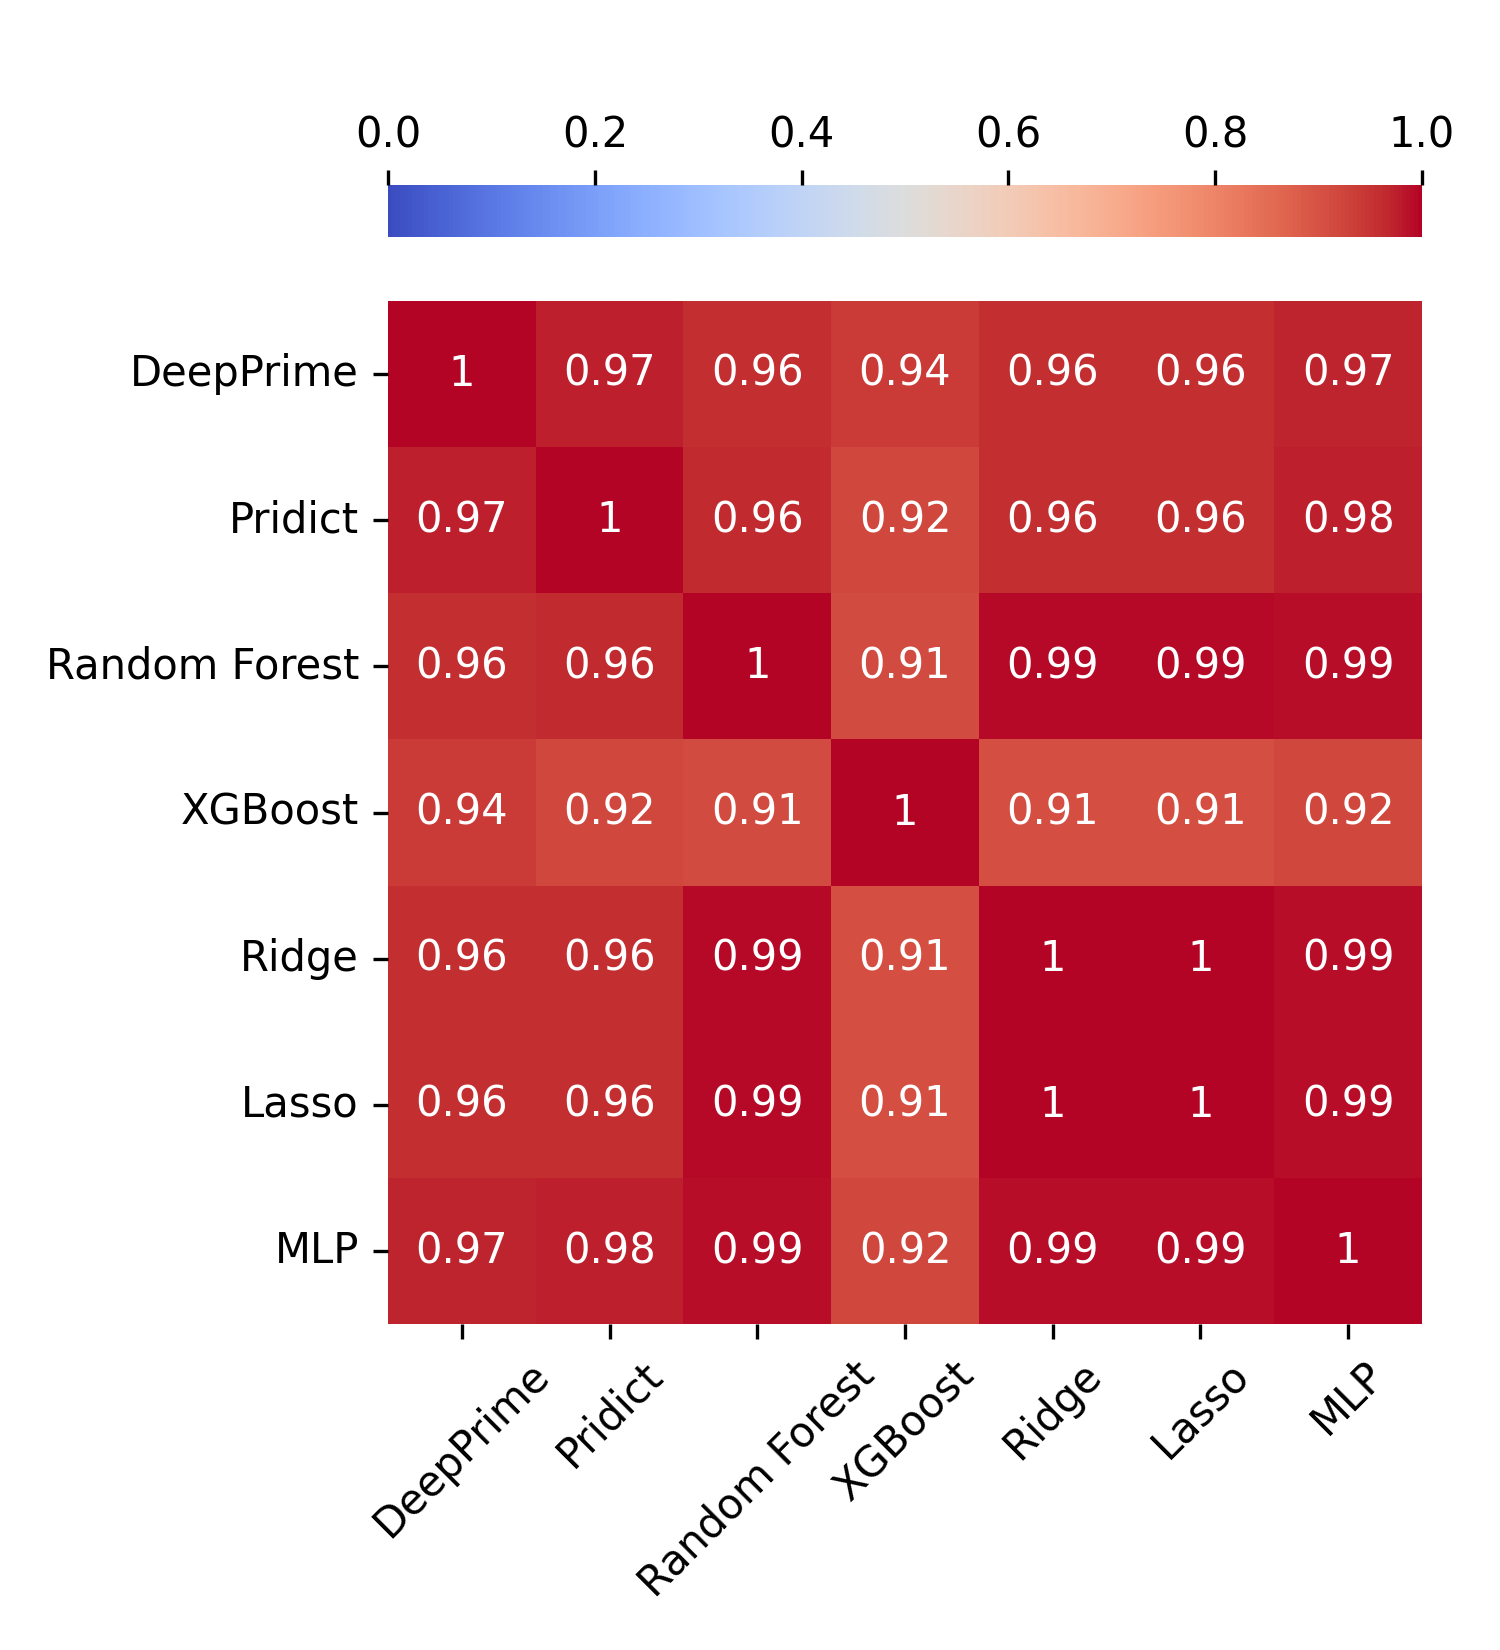
\includegraphics[width=0.49\textwidth]{error_correlation_pd-adv-pe2_pearson.png}
        % \caption{Pearson Correlation of the Error of the Individual Models}
        \label{fig:pearson-correlation-adv-pe2}
    }%
    \subfigure[][Spearman Correlation]{
        \centering
        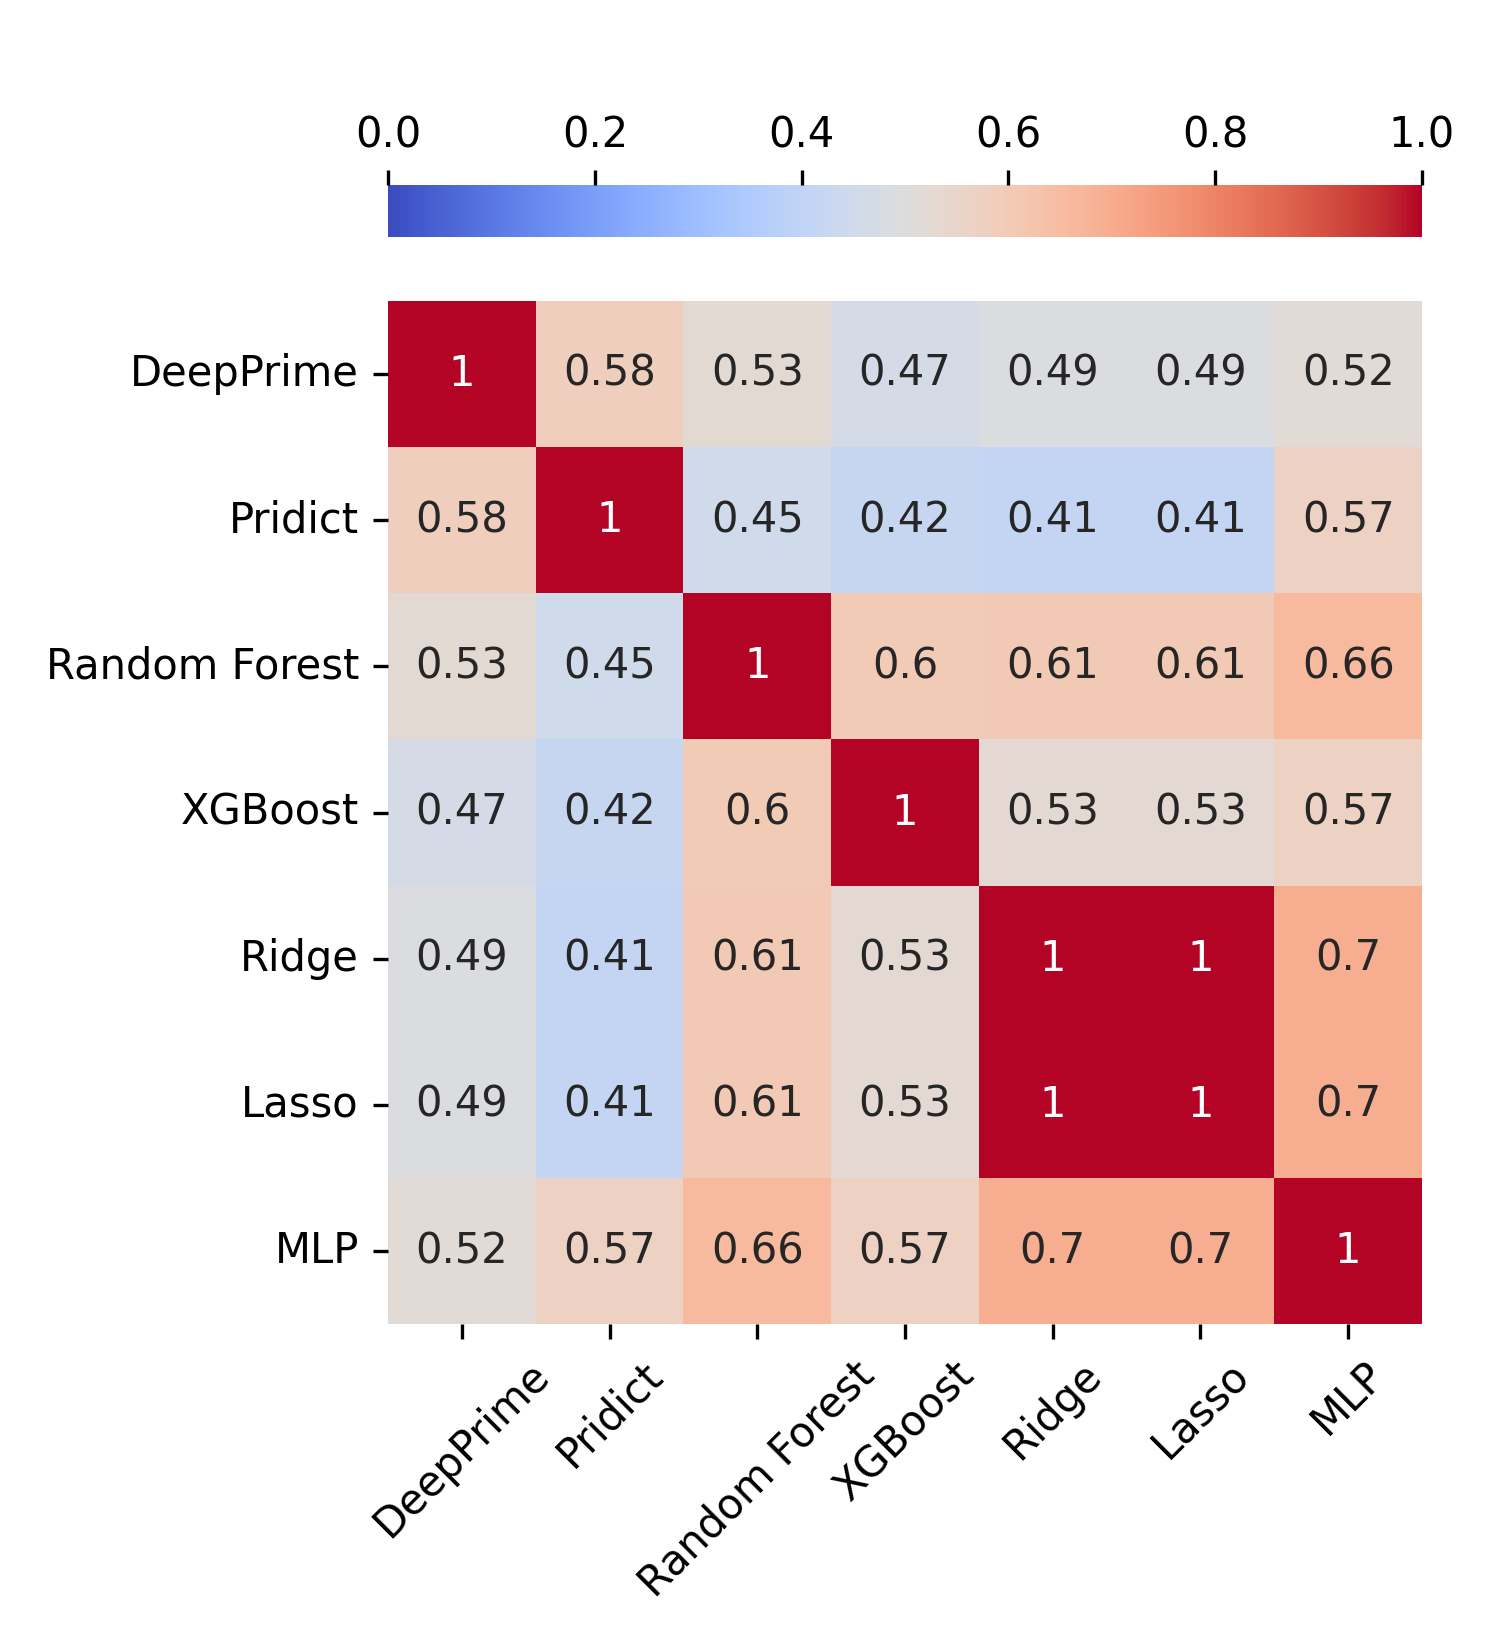
\includegraphics[width=0.49\textwidth]{error_correlation_pd-adv-pe2_spearman.png}
        % \caption{Spearman Correlation of the Error of the Individual Models}
        \label{fig:spearman-correlation-adv-pe2}
    }
    \caption[Error Analysis of the Individual Models on PRIDICT Adv PE2 dataset]{Error Analysis of the Individual Models on the PRIDICT Adv PE2 dataset. \textbf{(a)} The distribution of the error of the individual models at each example, smoothened using a moving window of size 100, and downsampled with a ratio of 10:1 for better visibility; \textbf{(b)} The Pearson correlation of the error of the individual models. \textbf{(c)} The Spearman correlation of the error of the individual models.}
    \label{fig:error-analysis-adv-pe2}
\end{figure}

The same error analysis conducted on \autoref{fig:error-analysis} was also conducted on the PRIDICT datasets. The result is very similar, but with major difference in terms of the correlation between PRIDICT and DeepPrime. The correlation between the two deep learning is much weaker, with the Spearman correlation around 0.7. The more dataset specific differences are pointed out in the caption of \autoref{fig:error-analysis-adv-pe2}, \autoref{fig:error-analysis-hek293t-pe2}, \autoref{fig:error-analysis-k562-pe2}, and \autoref{fig:error-analysis-k562mlh1dn-pe2}.

Due to the smaller data size, the downsampling and smoothing were done with a lower ratio of 10:1 and a smaller moving window of size 100, respectively. 

\begin{figure}
    \centering
    \subfigure[][Error Distribution]{
        \centering
        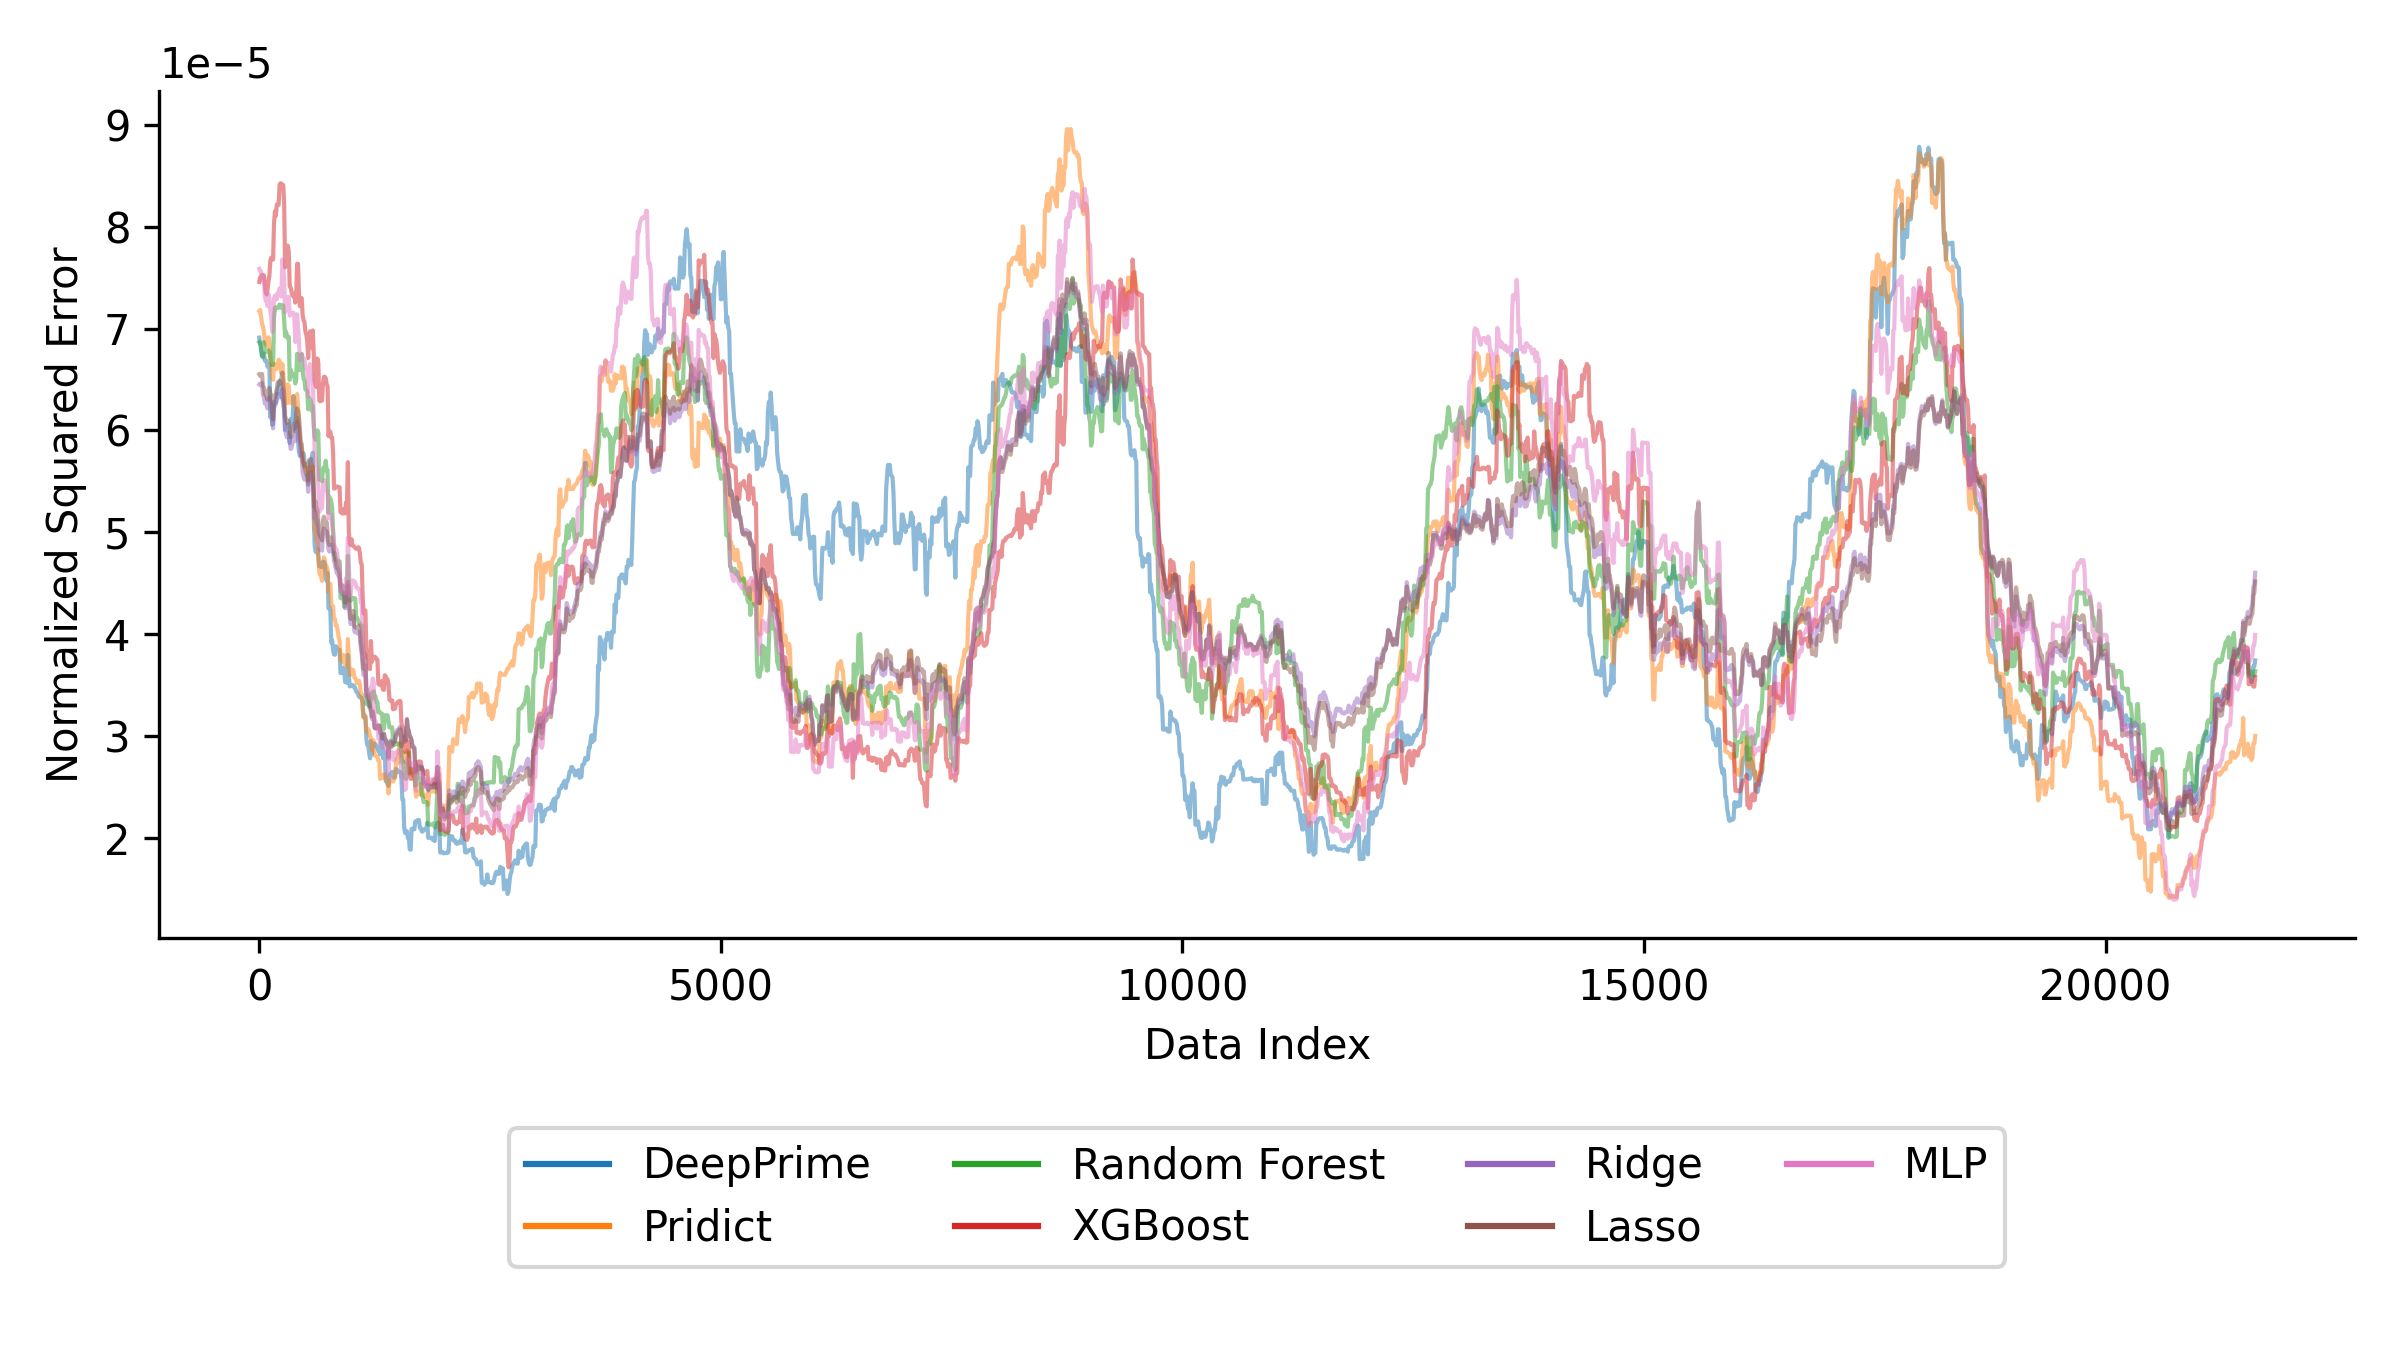
\includegraphics[width=\textwidth]{error_comparison_pd-hek293t-pe2.png}
        % \caption{Error Distribution of the Individual Models}
        \label{fig:error-distribution-hek293t-pe2}
    }
    \subfigure[][Pearson Correlation]{
        \centering
        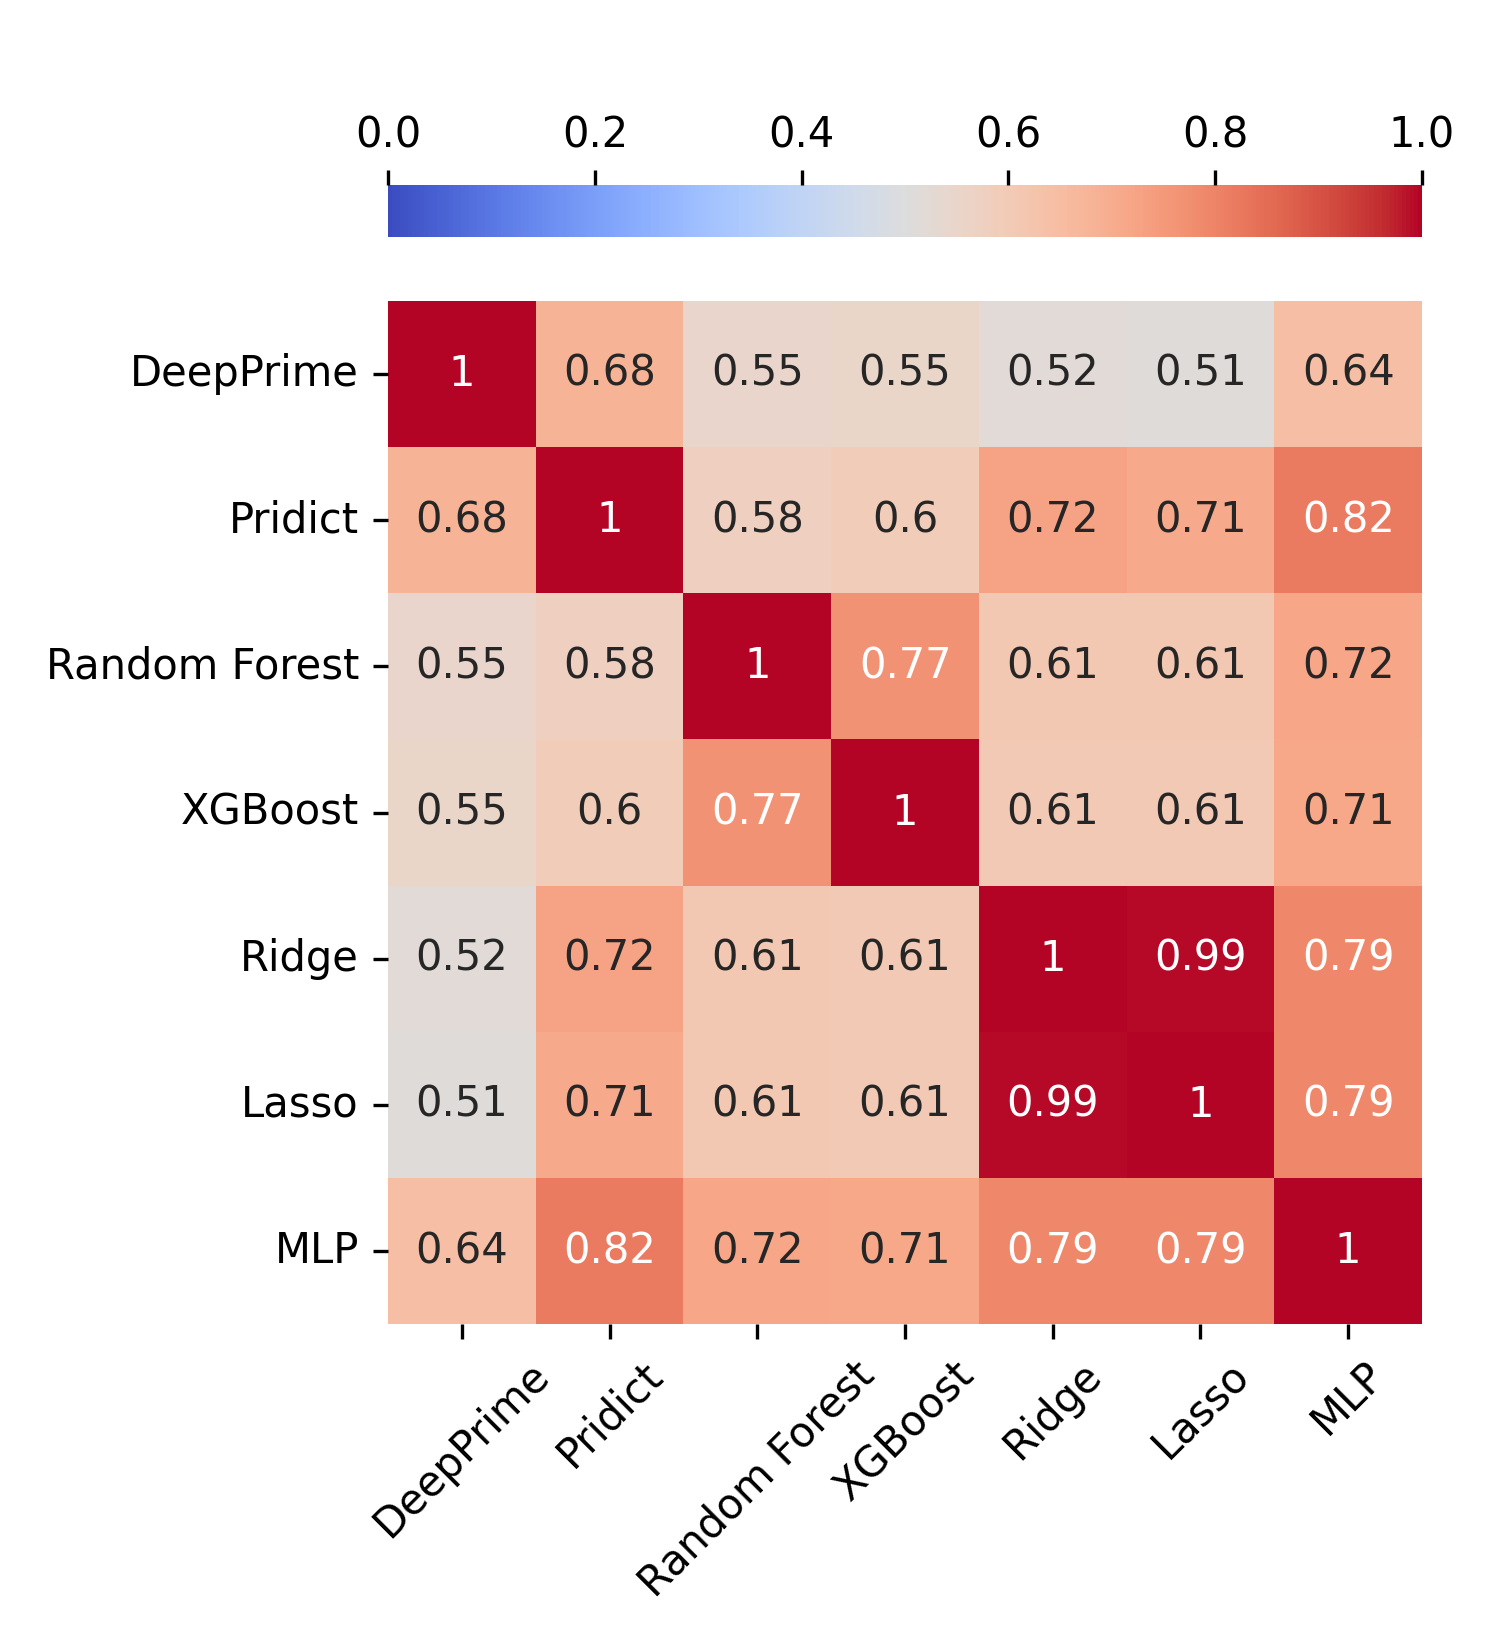
\includegraphics[width=0.49\textwidth]{error_correlation_pd-hek293t-pe2_pearson.png}
        % \caption{Pearson Correlation of the Error of the Individual Models}
        \label{fig:pearson-correlation-hek293t-pe2}
    }%
    \subfigure[][Spearman Correlation
    ]{
        \centering
        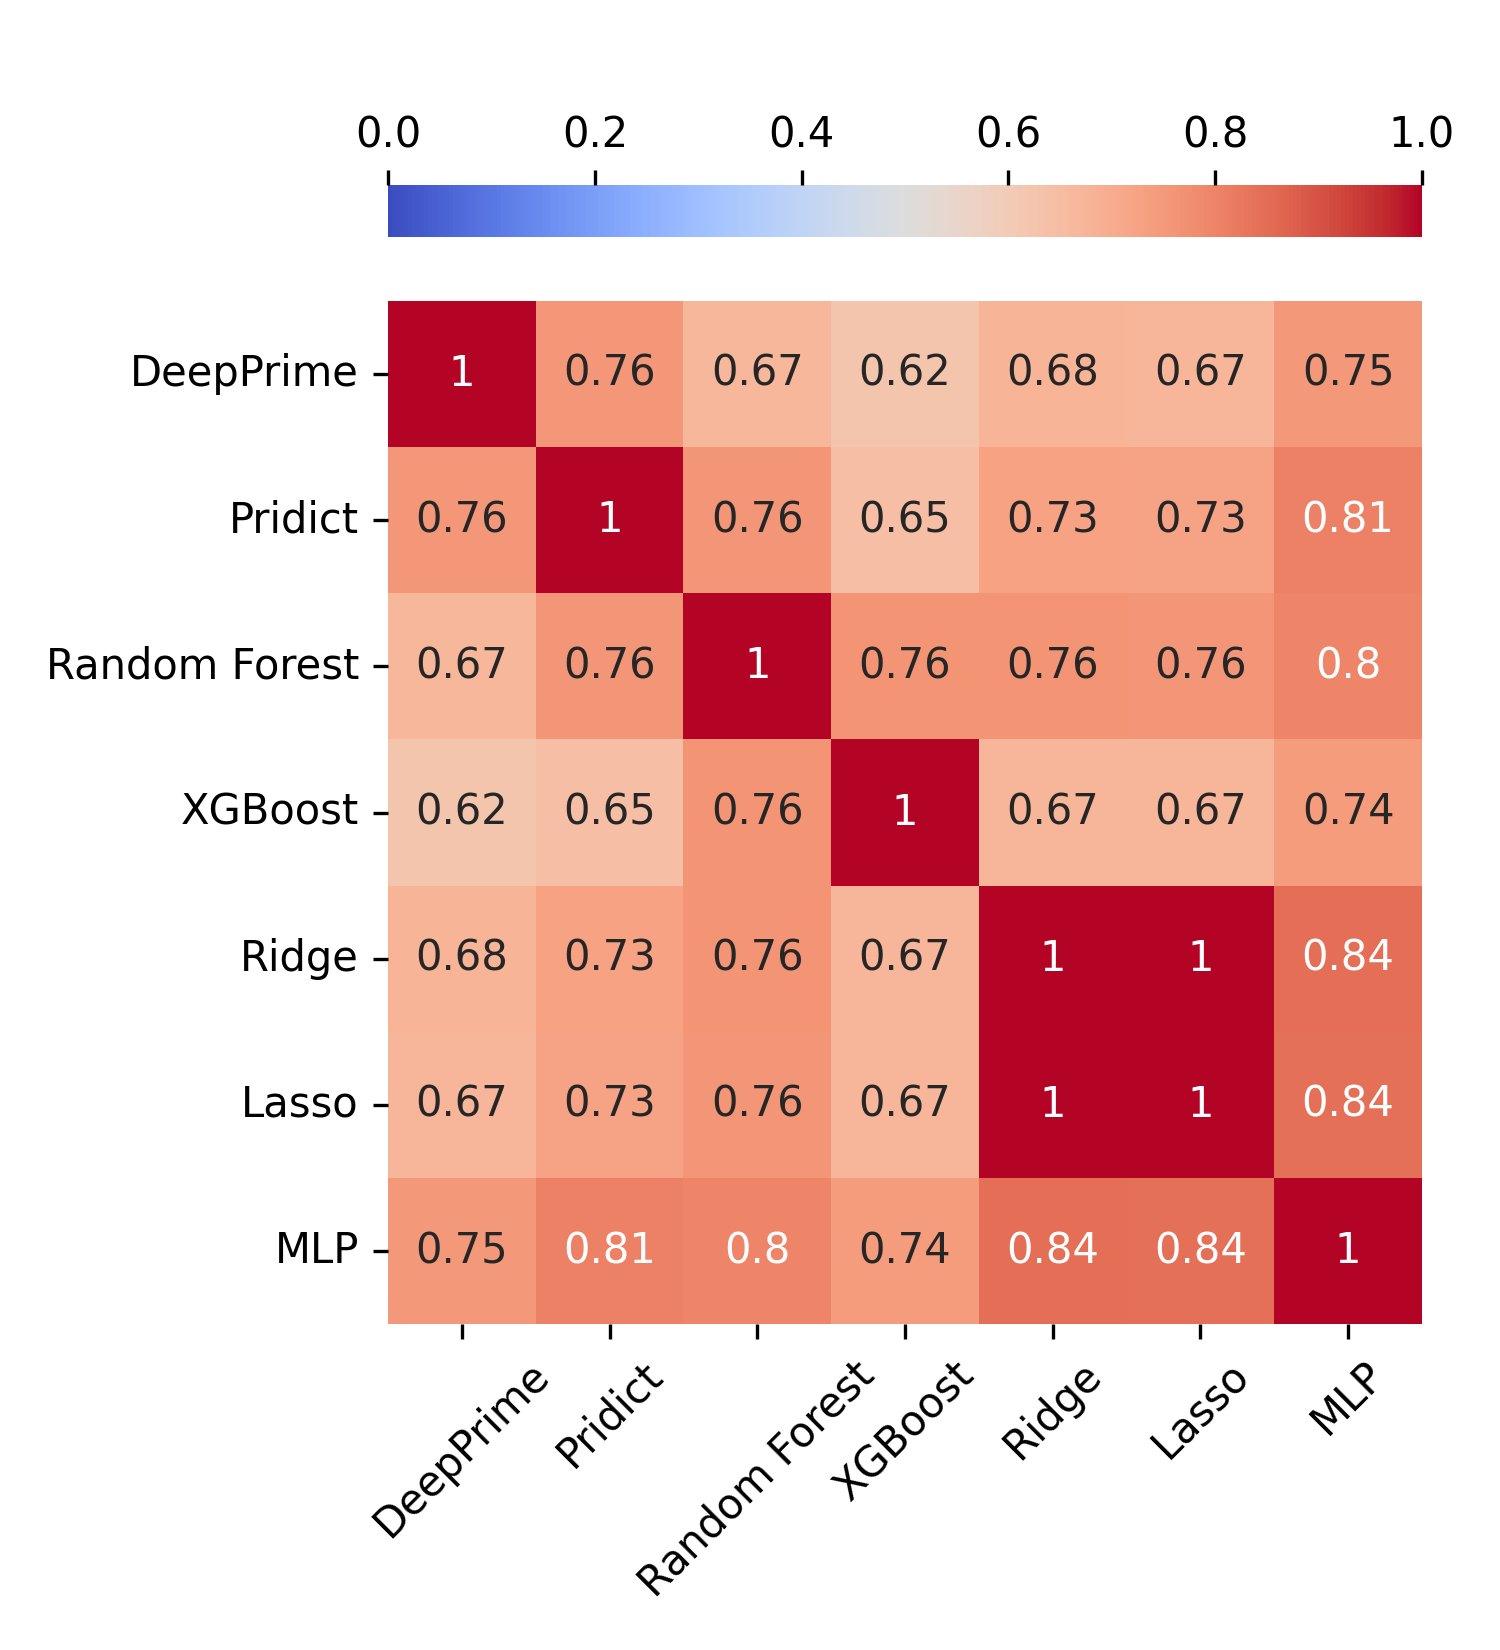
\includegraphics[width=0.49\textwidth]{error_correlation_pd-hek293t-pe2_spearman.png}
        % \caption{Spearman Correlation of the Error of the Individual Models}
        \label{fig:spearman-correlation-hek293t-pe2}
    }
    \caption[Error Analysis of the Individual Models on PRIDICT HEK293T PE2 dataset]{Error Analysis of the Individual Models on the PRIDICT HEK293T PE2 dataset. \textbf{(a)}, \textbf{(b)}, and \textbf{(c)} are the same as \autoref{fig:error-analysis-adv-pe2}. Pearson's r is much weaker, possibly due to a more balanced target value distribution as we have seen in \autoref{fig:imbalanced} The MLP is strongly correlated with all other models, especially PRIDICT.}
    \label{fig:error-analysis-hek293t-pe2}
\end{figure}

\begin{figure}
    \centering
    \subfigure[][Error Distribution]{
        \centering
        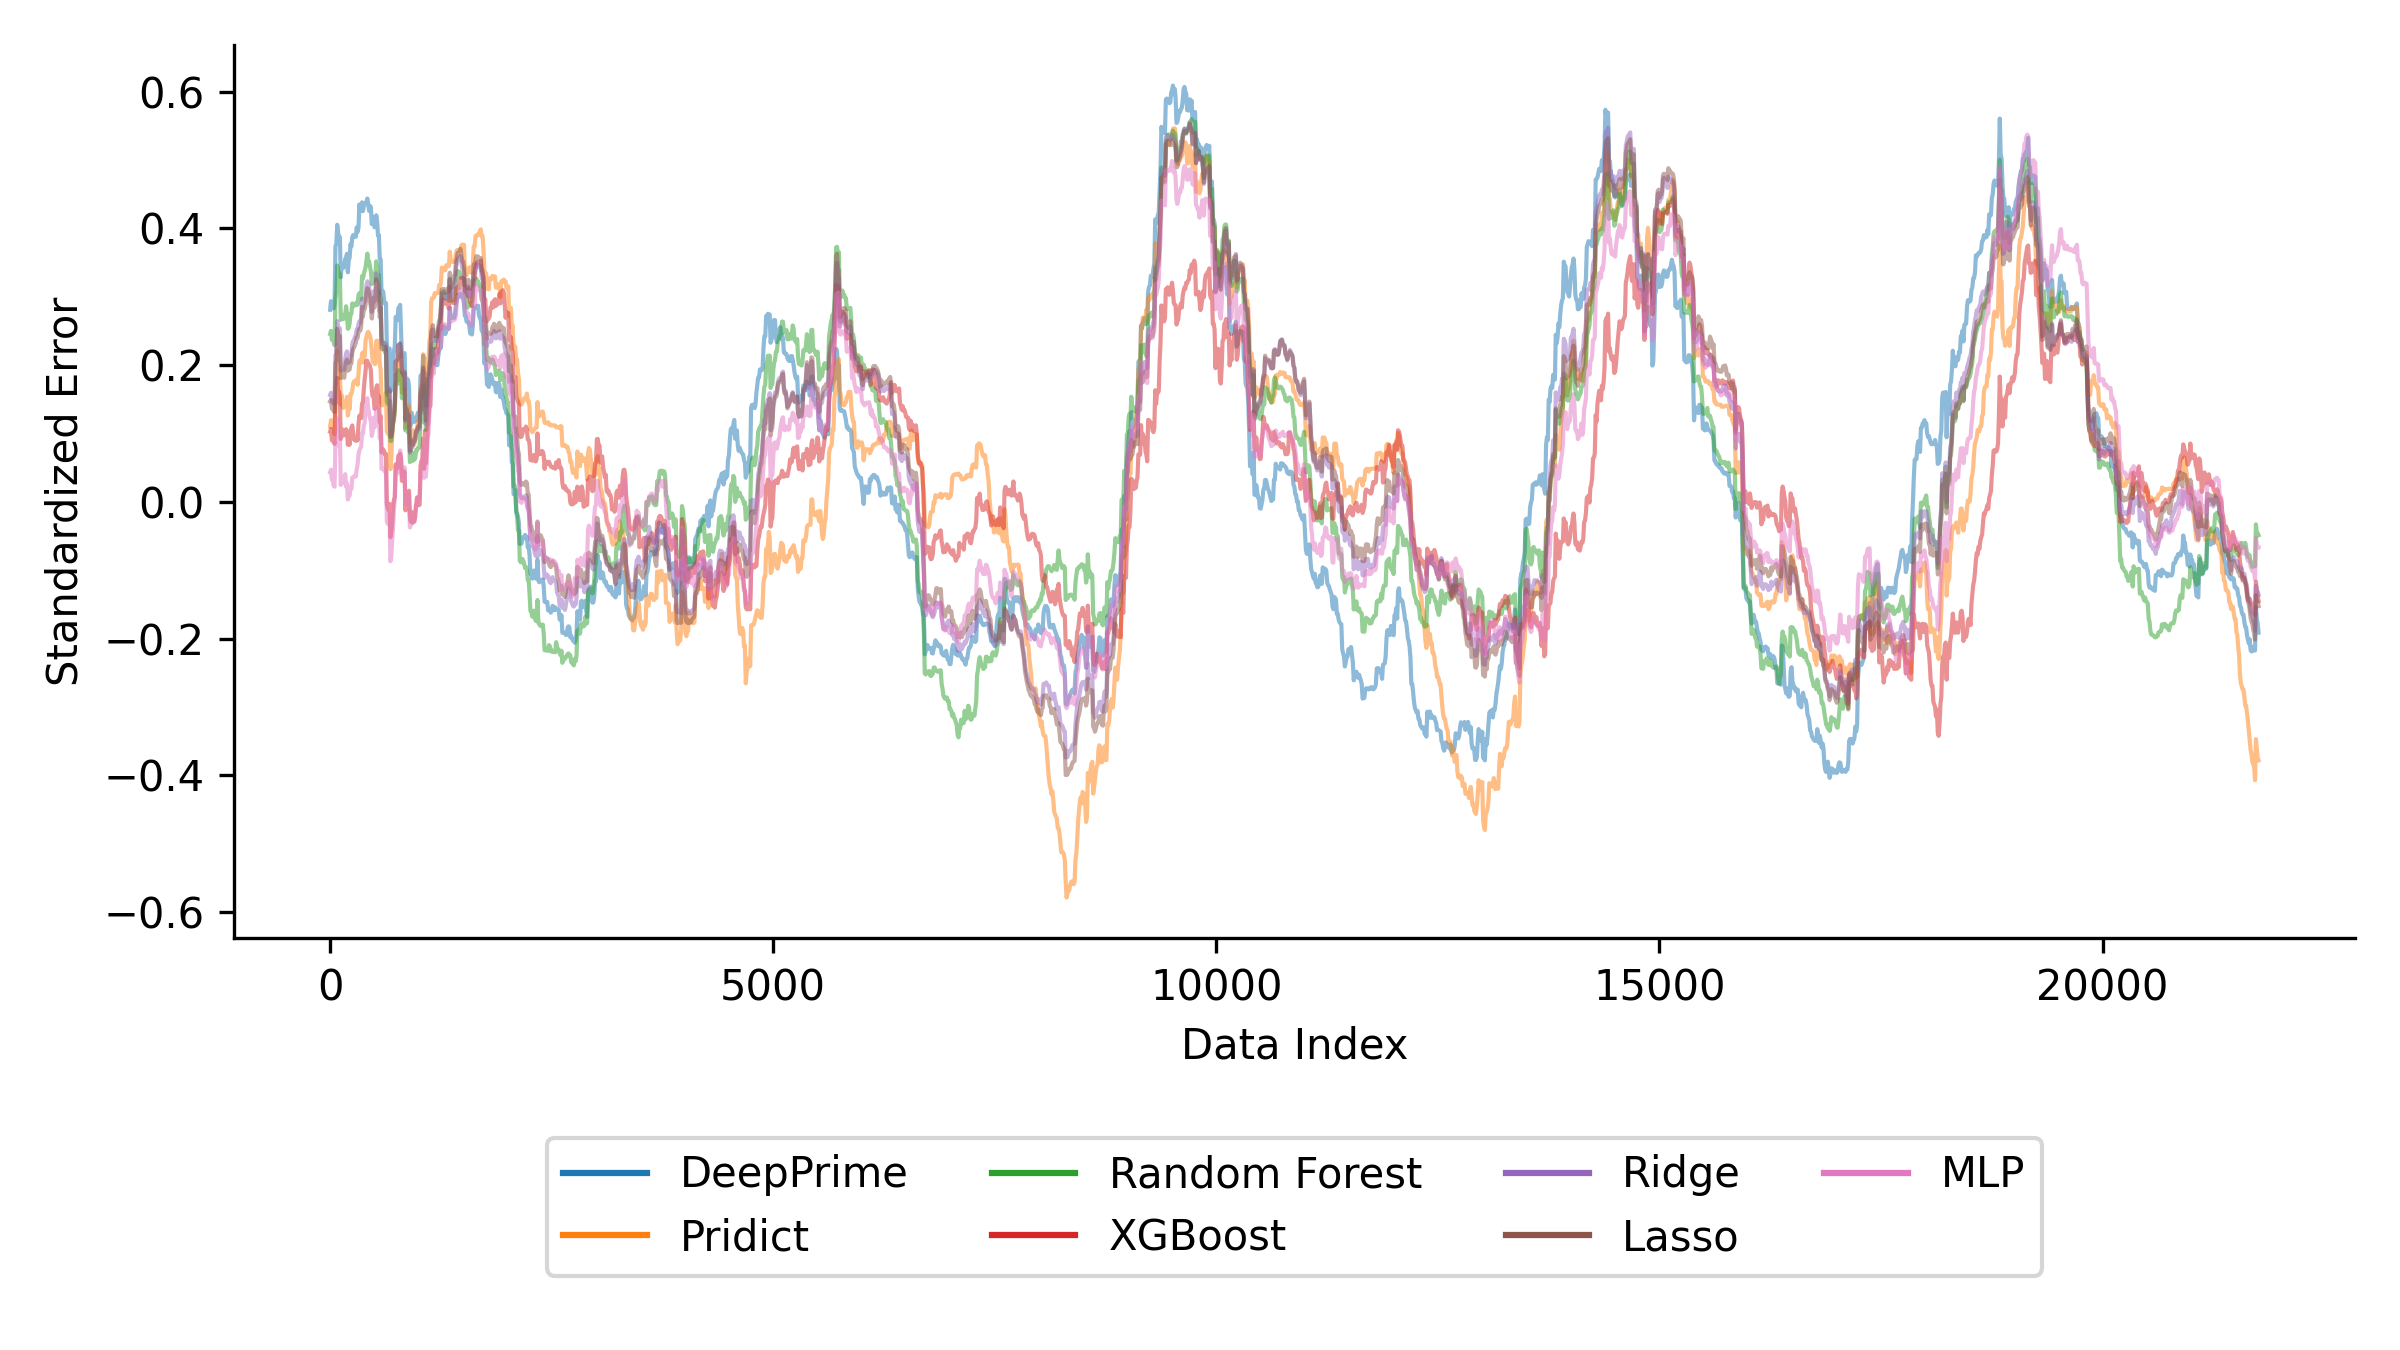
\includegraphics[width=\textwidth]{error_comparison_pd-k562-pe2.png}
        % \caption{Error Distribution of the Individual Models}
        \label{fig:error-distribution-k562-pe2}
    }
    \subfigure[][Pearson Correlation]{
        \centering
        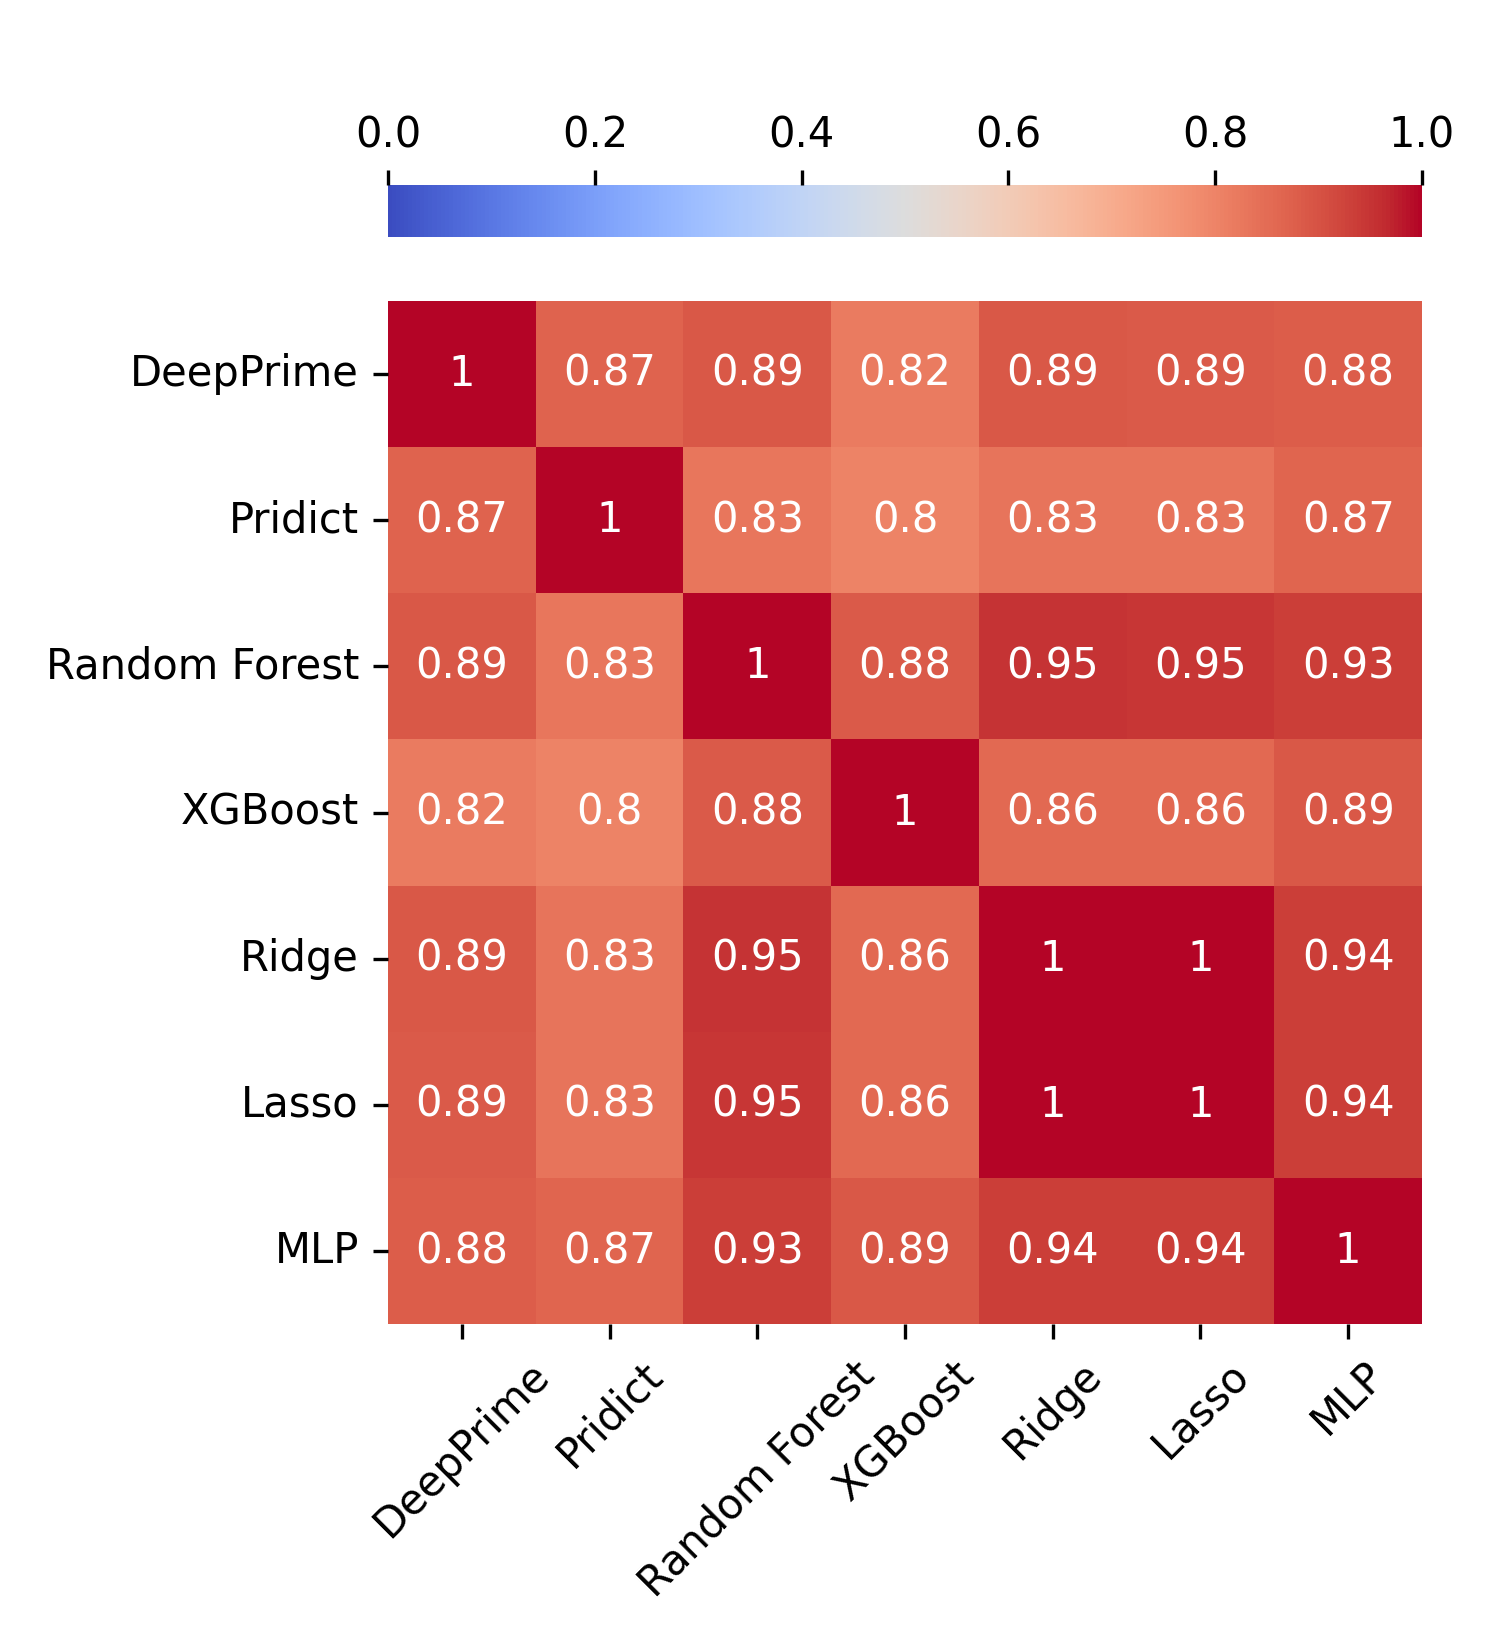
\includegraphics[width=0.49\textwidth]{error_correlation_pd-k562-pe2_pearson.png}
        % \caption{Pearson Correlation of the Error of the Individual Models}
        \label{fig:pearson-correlation-k562-pe2}
    }%
    \subfigure[][Spearman Correlation]{
        \centering
        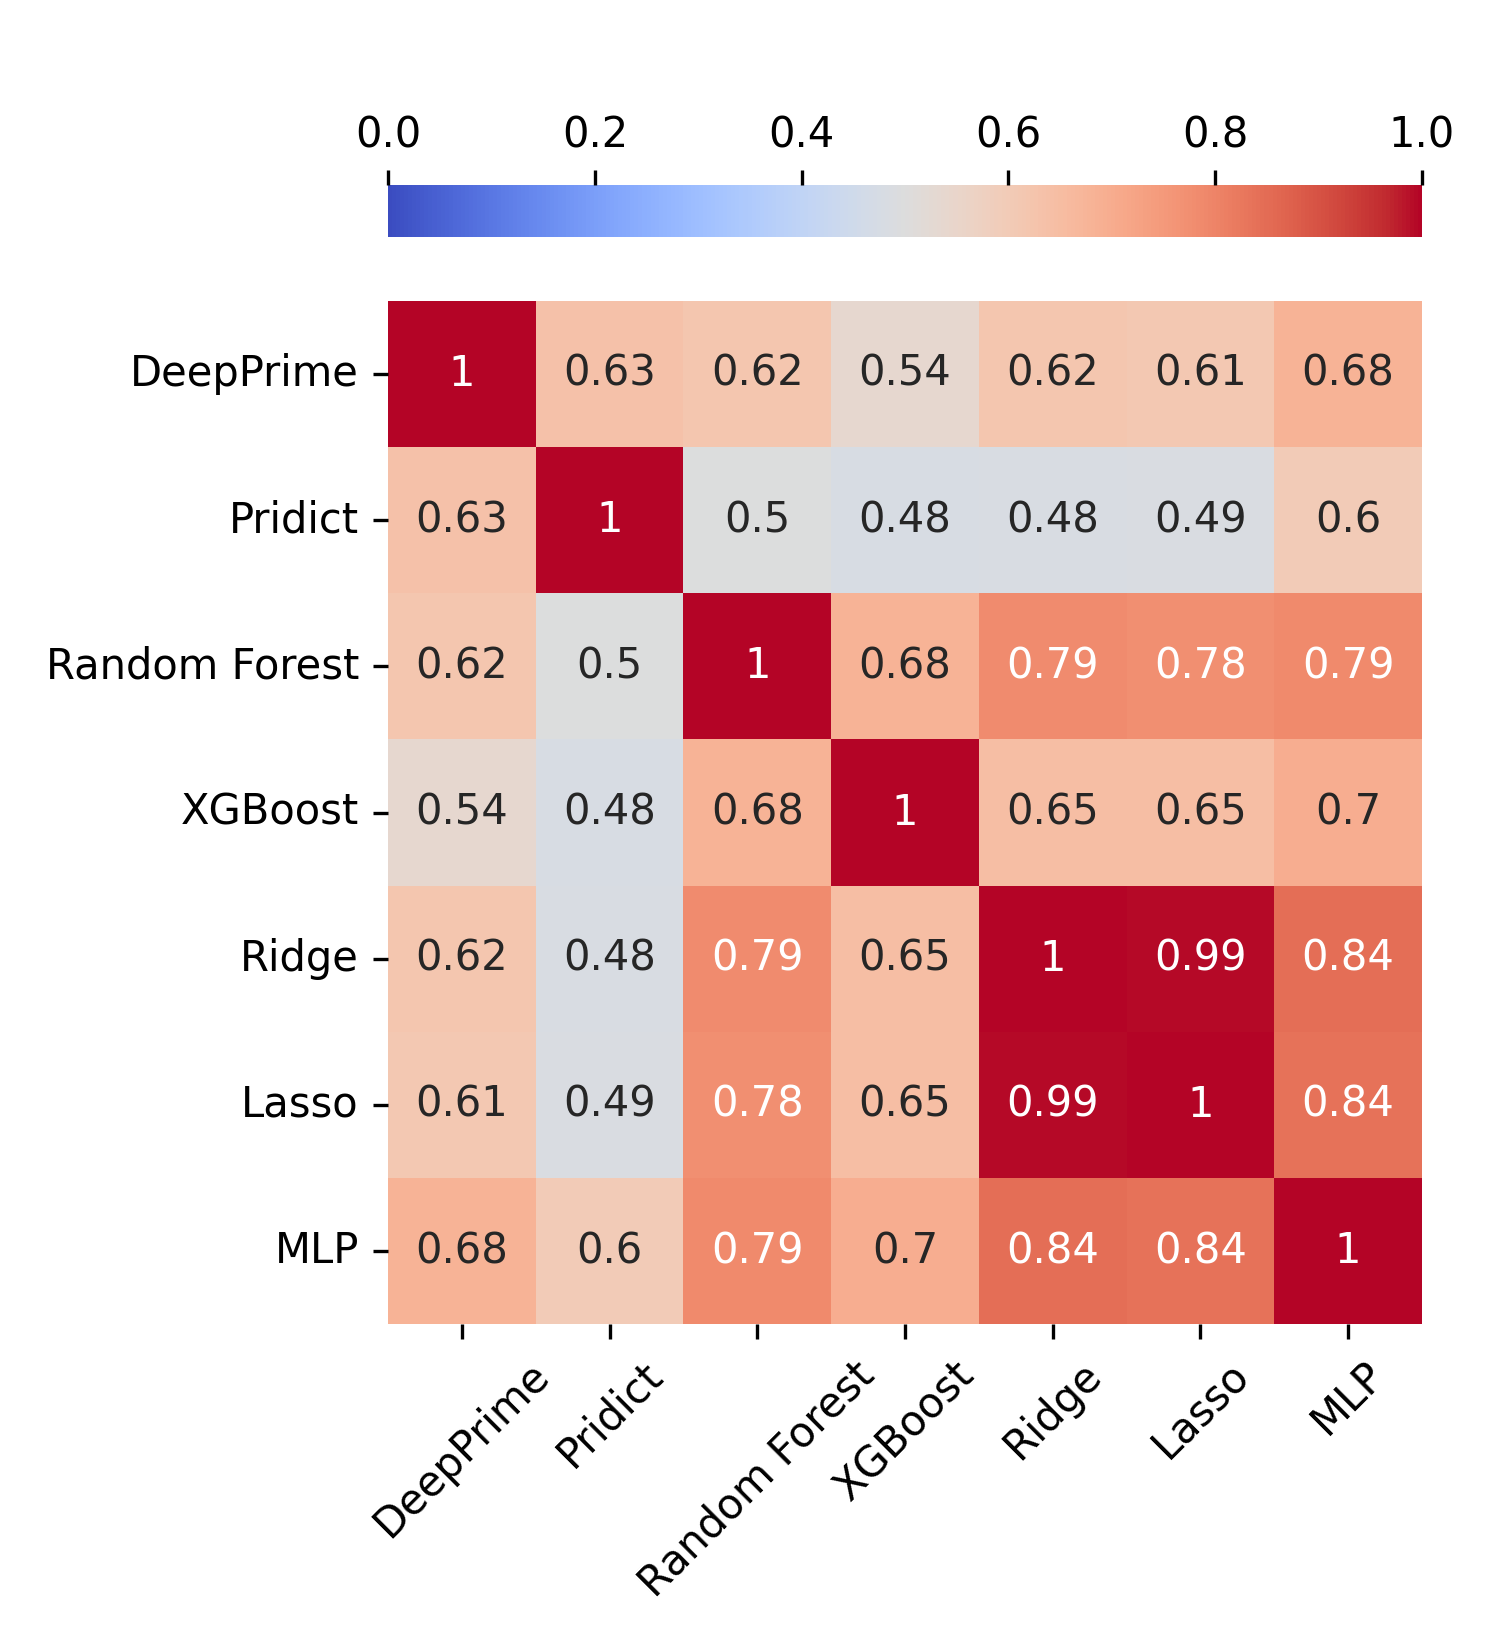
\includegraphics[width=0.49\textwidth]{error_correlation_pd-k562-pe2_spearman.png}
        % \caption{Spearman Correlation of the Error of the Individual Models}
        \label{fig:spearman-correlation-k562-pe2}
    }
    \caption[Error Analysis of the Individual Models on PRIDICT K562 PE2 dataset]{Error Analysis of the Individual Models on the PRIDICT K562 PE2 dataset. \textbf{(a)}, \textbf{(b)}, and \textbf{(c)} are the same as \autoref{fig:error-analysis-adv-pe2}.}
    \label{fig:error-analysis-k562-pe2}
\end{figure}

\begin{figure}
    \centering
    \subfigure[][Error Distribution]{
        \centering
        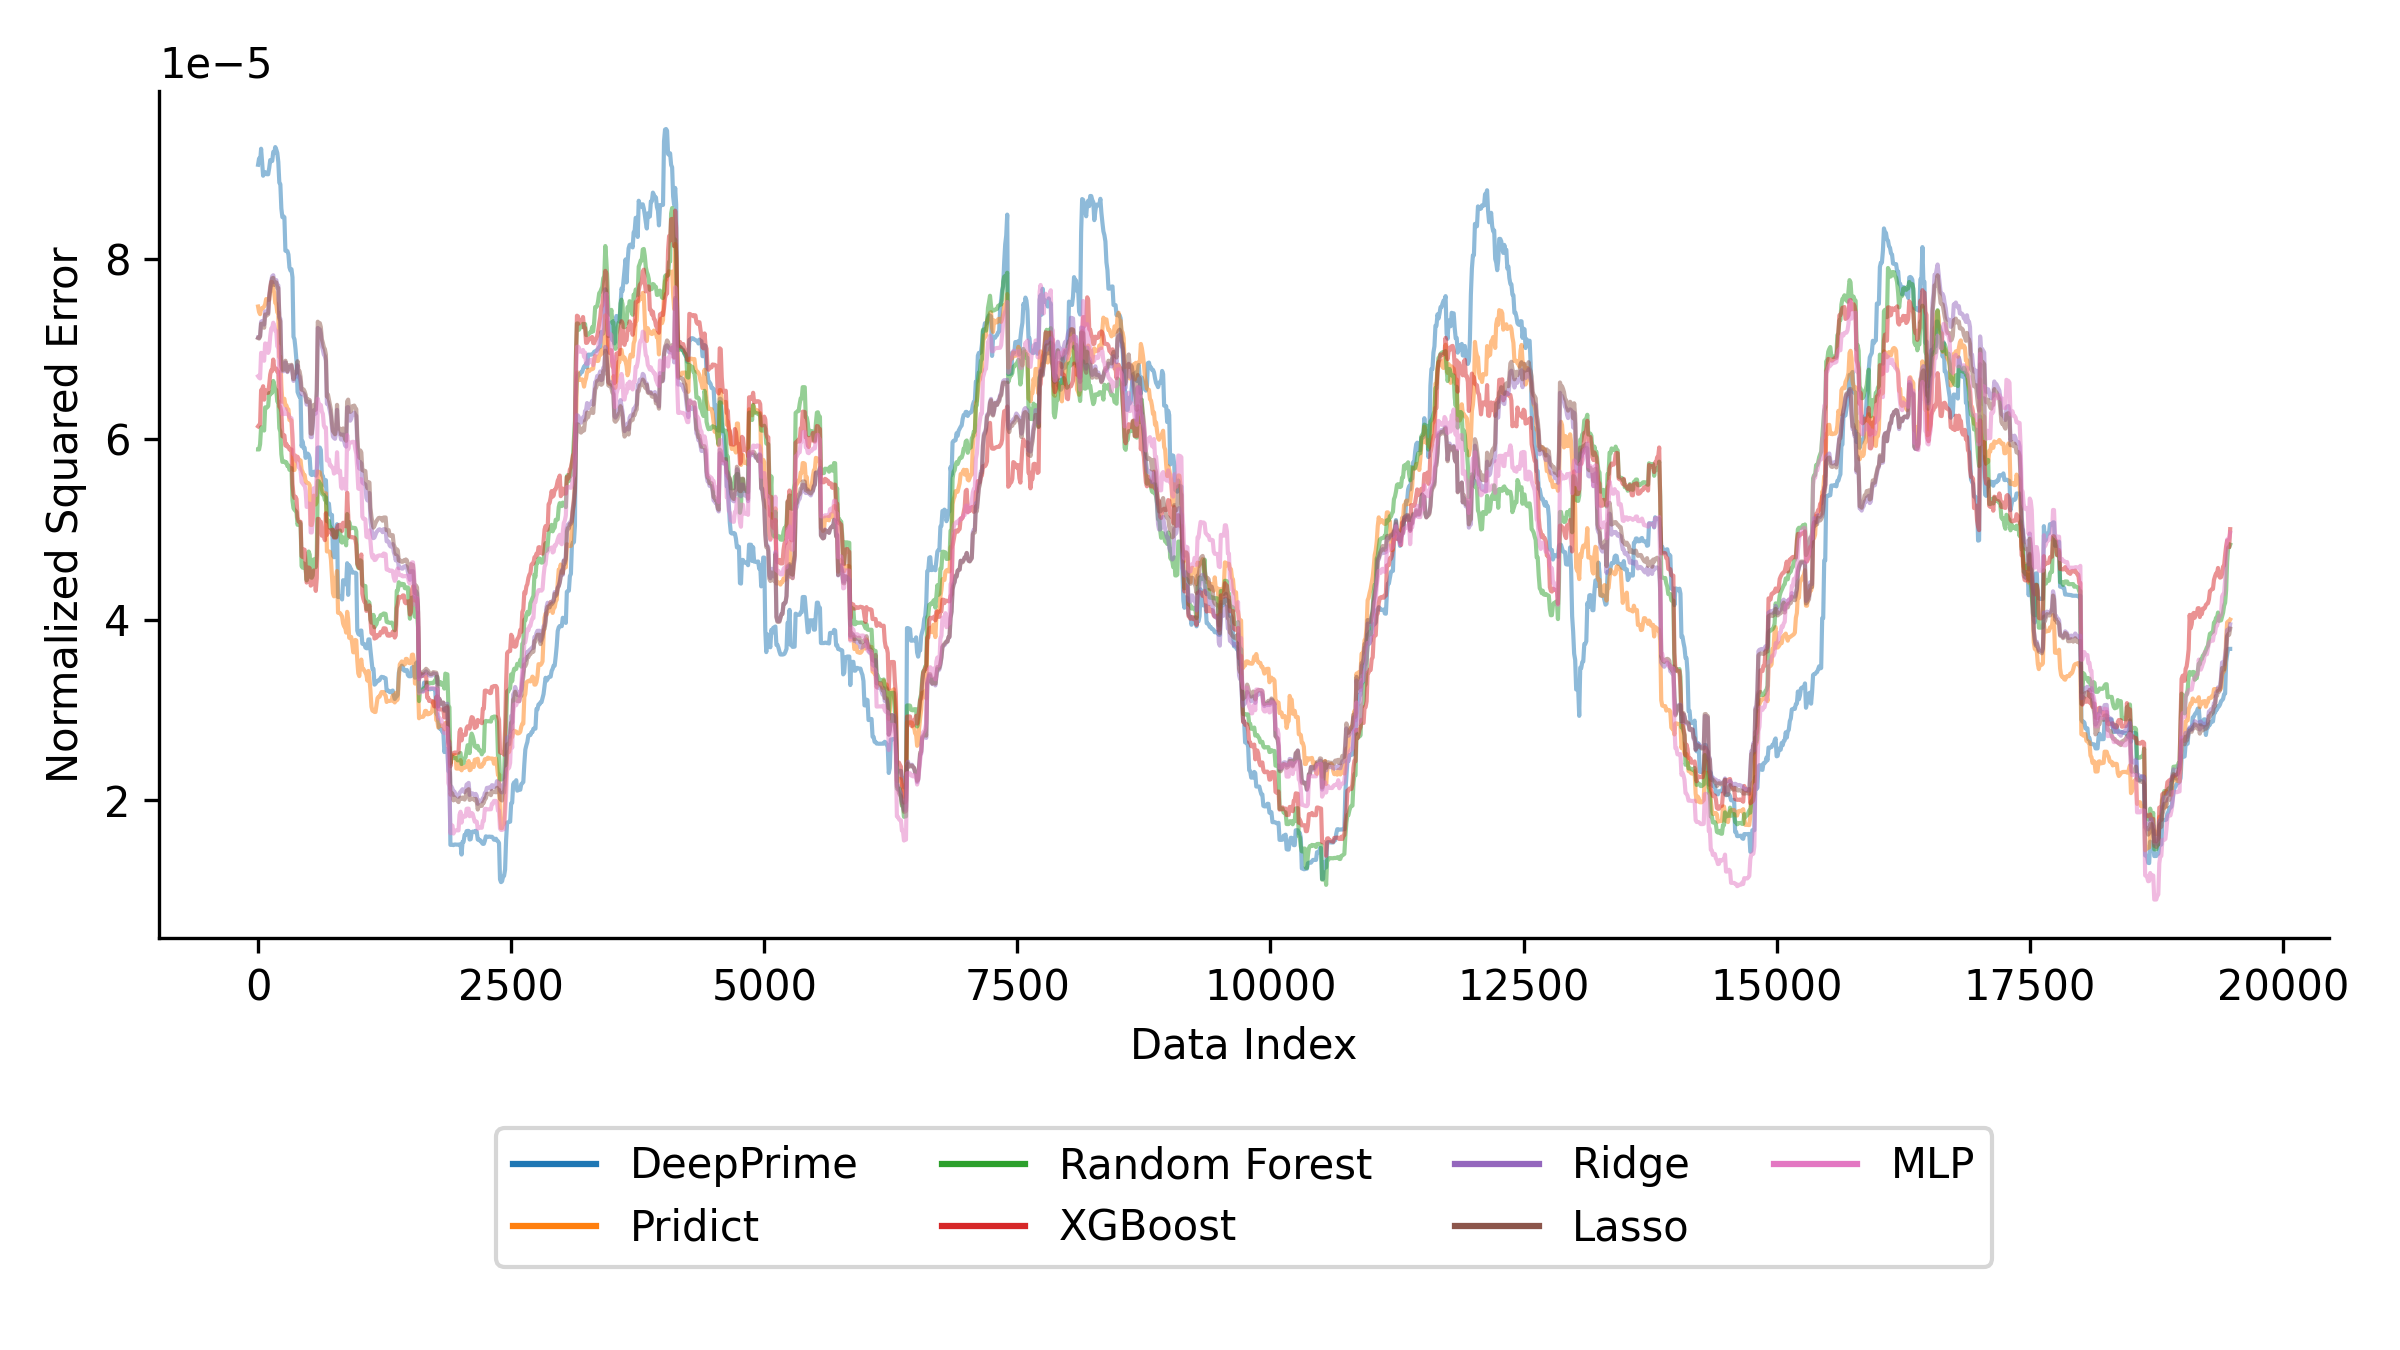
\includegraphics[width=\textwidth]{error_comparison_pd-k562mlh1dn-pe2.png}
        % \caption{Error Distribution of the Individual Models}
        \label{fig:error-distribution-k562mlh1dn-pe2}
    }
    \subfigure[][Pearson Correlation]{
        \centering
        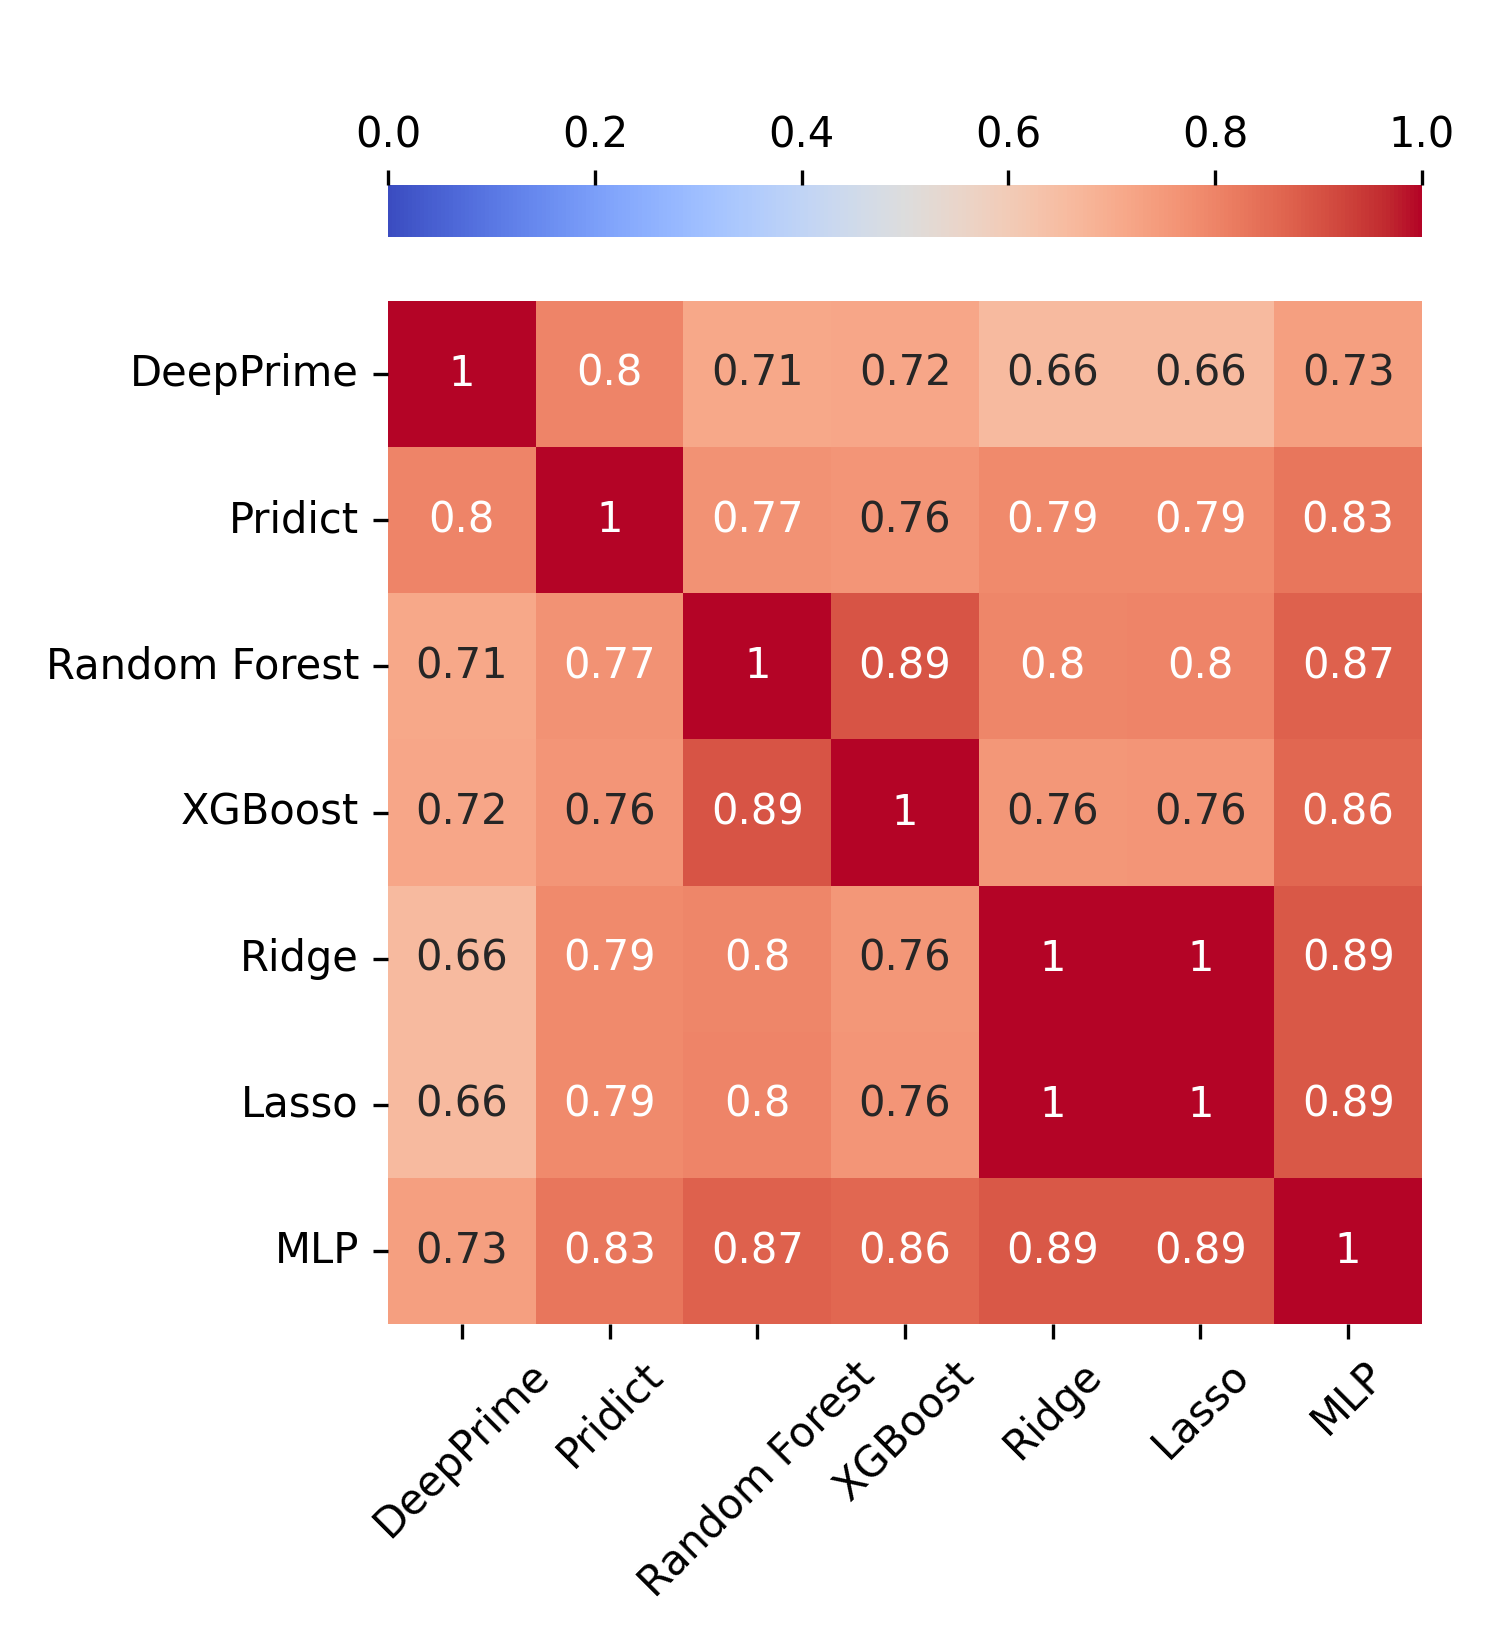
\includegraphics[width=0.49\textwidth]{error_correlation_pd-k562mlh1dn-pe2_pearson.png}
        % \caption{Pearson Correlation of the Error of the Individual Models}
        \label{fig:pearson-correlation-k562mlh1dn-pe2}
    }%
    \subfigure[][Spearman Correlation]{
        \centering
        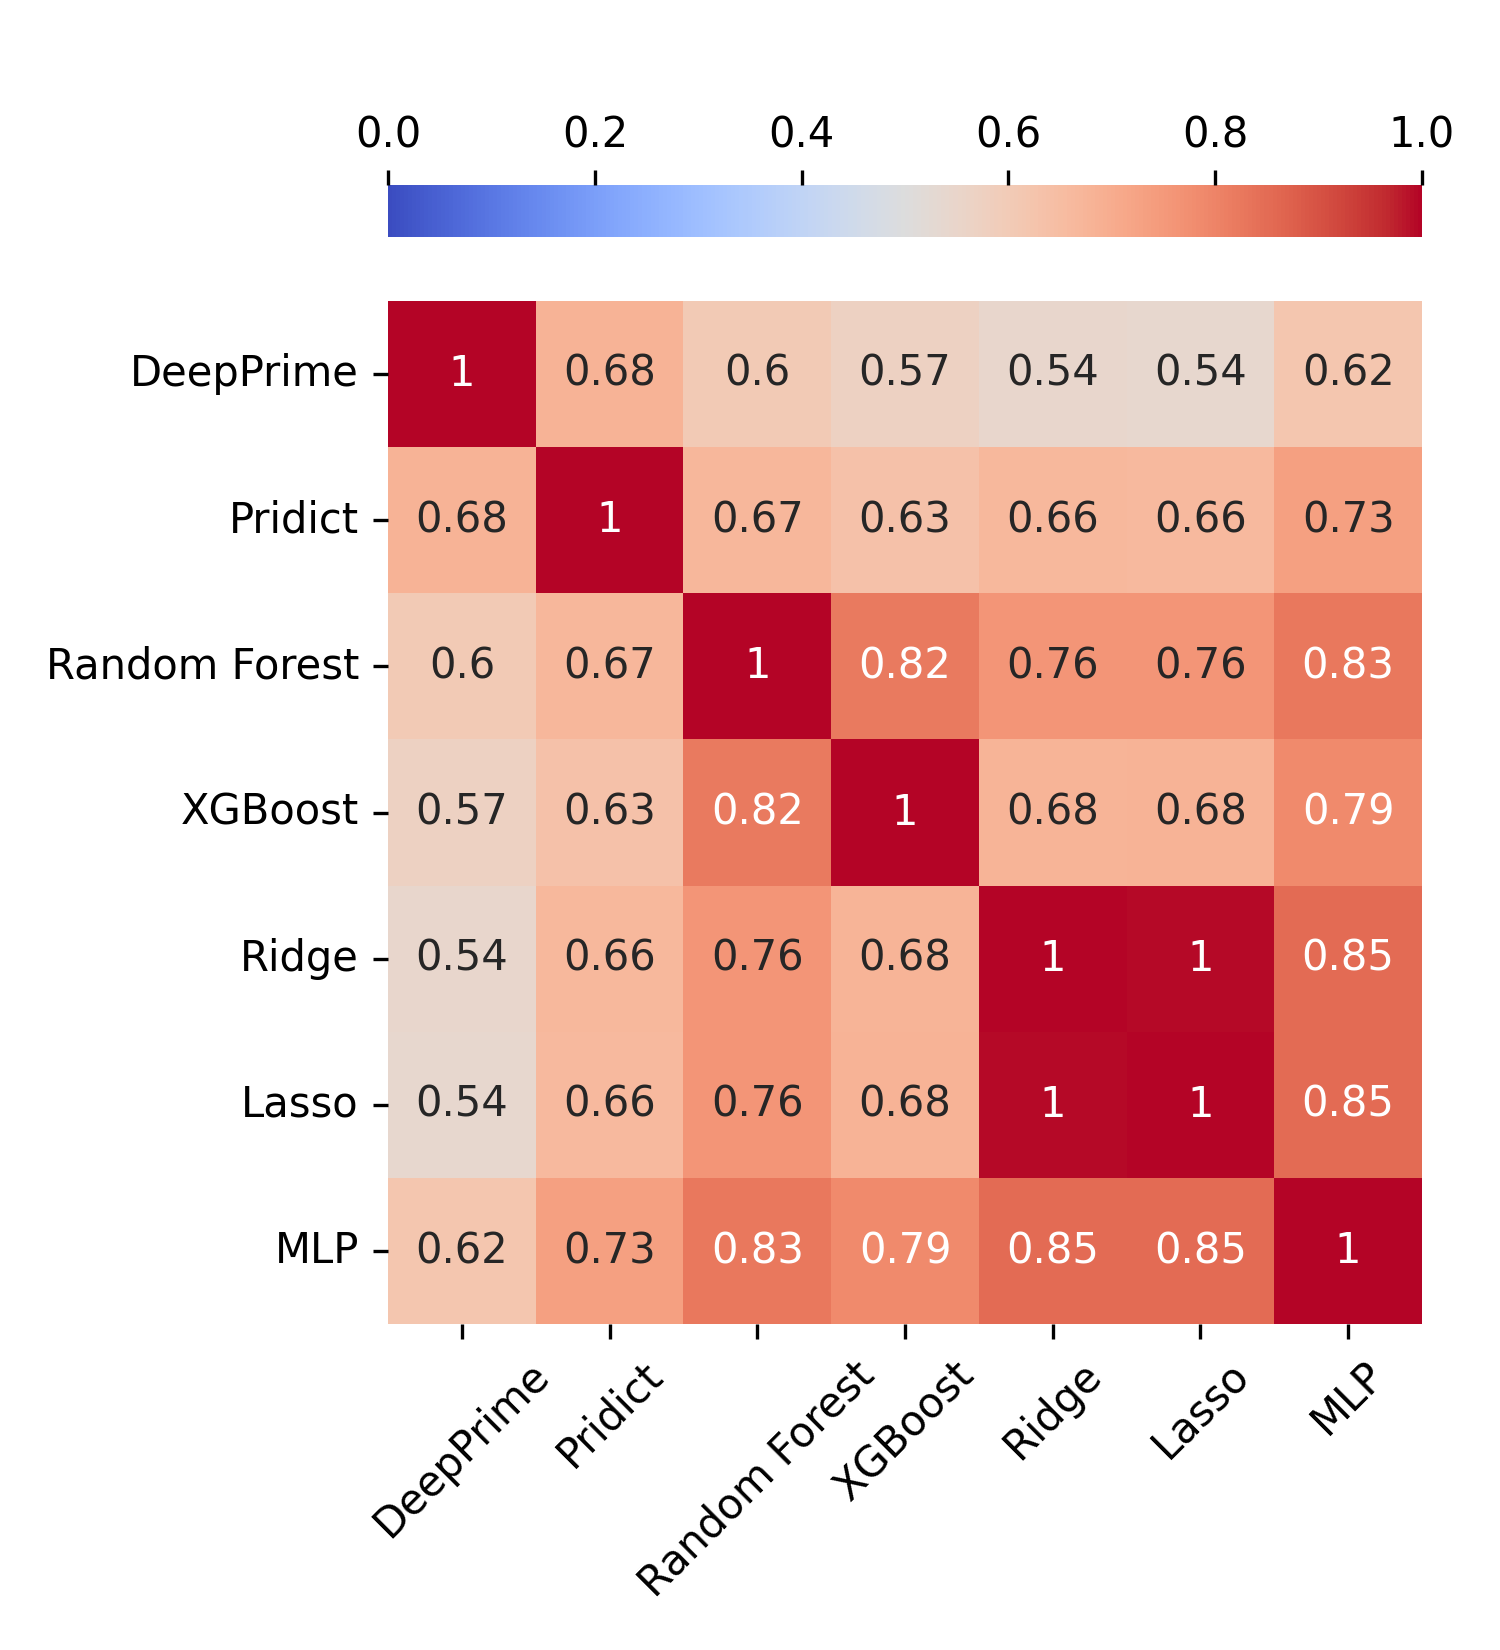
\includegraphics[width=0.49\textwidth]{error_correlation_pd-k562mlh1dn-pe2_spearman.png}
        % \caption{Spearman Correlation of the Error of the Individual Models}
        \label{fig:spearman-correlation-k562mlh1dn-pe2}
    }
    \caption[Error Analysis of the Individual Models on PRIDICT K562 MLH1 DN PE2 dataset]{Error Analysis of the Individual Models on the PRIDICT K562 MLH1 DN PE2 dataset. \textbf{(a)}, \textbf{(b)}, and \textbf{(c)} are the same as \autoref{fig:error-analysis-adv-pe2}.}
    \label{fig:error-analysis-k562mlh1dn-pe2}
\end{figure}

\begin{figure}
    
\end{figure}

\section{}